\documentclass[notes=show]{beamer}
\usepackage{mathpazo}
\usepackage{hyperref}
\usepackage{multimedia}
\usepackage{tcolorbox}
\usepackage{tikz}
\usetikzlibrary{shadows}
\usetheme{metropolis}
\usecolortheme{default}
\setbeamertemplate{itemize item}{%
    
\begin{tikzpicture}
        \shade[ball color=black!100!yellow, preaction={fill=black,
opacity=.00,transform canvas={xshift=1mm,yshift=-1mm, yscale=0.5}}] (0,0) circle (0.6ex);
    \end{tikzpicture}
}
\setbeamertemplate{itemize subitem}{%
    
\begin{tikzpicture}
        \shade[ball color=black!100!white, preaction={fill=black,
        opacity=.00,transform canvas={xshift=1mm,yshift=-1mm, yscale=0.5}}] (0,0) circle (0.6ex);
    \end{tikzpicture}
}
\setbeamercolor{frametitle}{bg=white}
\setbeamercolor{frametitle}{fg=black}
\setbeamercolor{background canvas}{bg=white}
\setbeamercolor{block body}{bg=mDarkTeal!30}
\setbeamercolor{block title}{bg=mDarkTeal,fg=black!2}
\setbeamertemplate{navigation symbols}{}
\setbeamertemplate{footline}[page number]
\newenvironment{stepenumerate}{\begin{enumerate}[<+->]}{\end{enumerate}}
\newenvironment{stepitemize}{\begin{itemize}[<+->]}{\end{itemize} }
\newenvironment{stepenumeratewithalert}{\begin{enumerate}[<+-| alert@+>]}{\end{enumerate}}
\newenvironment{stepitemizewithalert}{\begin{itemize}[<+-| alert@+>]}{\end{itemize} }

\begin{document}

\title[Skill, Tasks and Technologies]{Skills, Tasks and Technologies: Implications for Employment and Earnings}
\subtitle{}
\date{Daron Acemoglu \& David Autor \bigskip \\
\textit{Handbook of Labor Economics}, January 2011, Part 1, pages 1044-1118}
\author{}
\maketitle

\begin{frame}{Table of Contents}
\begin{itemize}
\item[1.] Introduction \medskip
\item[2.] An Overview of Labor Market Trends \medskip
\item[3.] The Canonical Model \medskip
\item[\textcolor{gray}{4.}] \textcolor{gray}{A Ricardian Model of the Labor Market} \medskip
\item[\textcolor{gray}{5.}] \textcolor{gray}{Comparative Advantange and Wages: An Empirical Approach} \medskip
\item[\textcolor{gray}{6.}] \textcolor{gray}{Concluding Remarks}
\end{itemize}
\end{frame}

\section{1. Introduction}

\begin{frame}{Introduction}
\begin{itemize}
\item This chapter presents an overview of labor market trends. \bigskip
\item It summarizes the canonical model, tractable and conceptually attractive, that has been successful in explaining most of these trends. \bigskip
\item However, some recent trends necessitate a richer framework.\bigskip
\item To this end, the chapter develops a Ricardian model of Roy-type self-selection of workers into tasks.
\end{itemize}
\end{frame}

\section{2. An Overview of Labor Market Trends}

\begin{frame}{2. An overview of labor market trends}
\begin{itemize}
\item[\textcolor{red}{2.1}] \textcolor{red}{A brief overview of data sources} \medskip
\item[\textcolor{gray}{2.2}] \textcolor{gray}{The college/high school wage premium} \medskip
\item[\textcolor{gray}{2.3}] \textcolor{gray}{Real wage levels by skill group} \medskip
\item[\textcolor{gray}{2.4}] \textcolor{gray}{Overall wage inequality} \medskip
\item [\textcolor{gray}{2.5}] \textcolor{gray}{Job polarization}
\end{itemize}
\end{frame}

\subsection{2.1 A brief overview of data sources}

\begin{frame}{A brief overview of data sources}
\begin{enumerate}
\item \underline{March Current Population Survey (March CPS)}: \linebreak
Average weekly earnings and employment in past year for FTFY workers, 1963-2008. \smallskip
\item \underline{May/ORG Current Population Survey (MORG CPS)}: \linebreak
Hourly wages and employment in survey week for all wage and salary workers, 1973-2009. \smallskip
\item \underline{Census of Populations (Census)}: \linebreak
Wages and employment as March CPS for 1\% sample of US population in 1960 and 1970 and 5\% sample in 1980, 1990, 2000, larger samples suited for detailed occupational analyses.\smallskip
\item \underline{American Community Survey (ACS)}: \linebreak
As Census for 2008.
\end{enumerate}
\end{frame}

\subsection{2.2 The college/high school wage premium}

\begin{frame}{2. An overview of labor market trends}
\begin{itemize}
\item[\textcolor{gray}{2.1}] \textcolor{gray}{A brief overview of data sources} \medskip
\item[\textcolor{red}{2.2}] \textcolor{red}{The college/high school wage premium} \medskip
\item[\textcolor{gray}{2.3}] \textcolor{gray}{Real wage levels by skill group} \medskip
\item[\textcolor{gray}{2.4}] \textcolor{gray}{Overall wage inequality} \medskip
\item [\textcolor{gray}{2.5}] \textcolor{gray}{Job polarization}
\end{itemize}
\end{frame}

\newpage
\begin{center}
\begin{figure}
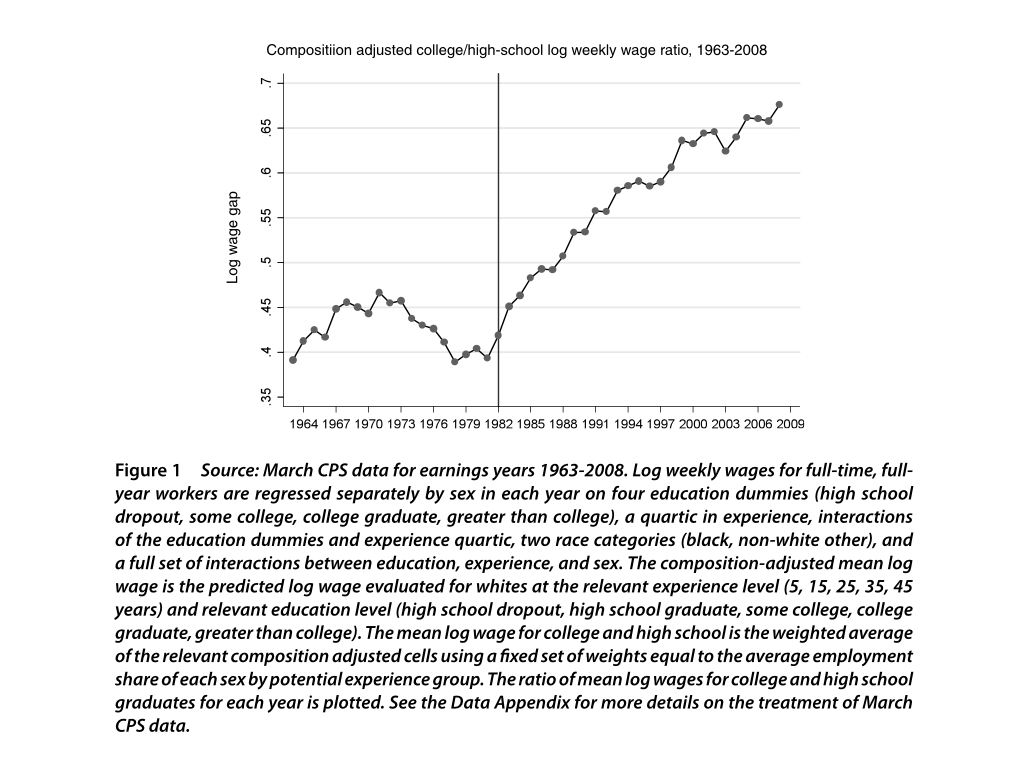
\includegraphics[height=8.5cm,width=\textwidth]{figure1.png}
\end{figure} 
\end{center}
\newpage

\begin{frame}{The college/high school wage premium (Figure 1)}
\begin{enumerate}
\item In 2008, the college premium stood at a maximum 68 log points (or $\exp(0.68) - 1 \approx 0.97$ or 97\%). \bigskip
\item The college premium declined between 1971 and 1978 and increased afterwards. \bigskip
\item This is critical to our understanding of supply and demand in the determination of between-group wage inequality.
\end{enumerate}
\end{frame}

\newpage
\begin{center}
\begin{figure}
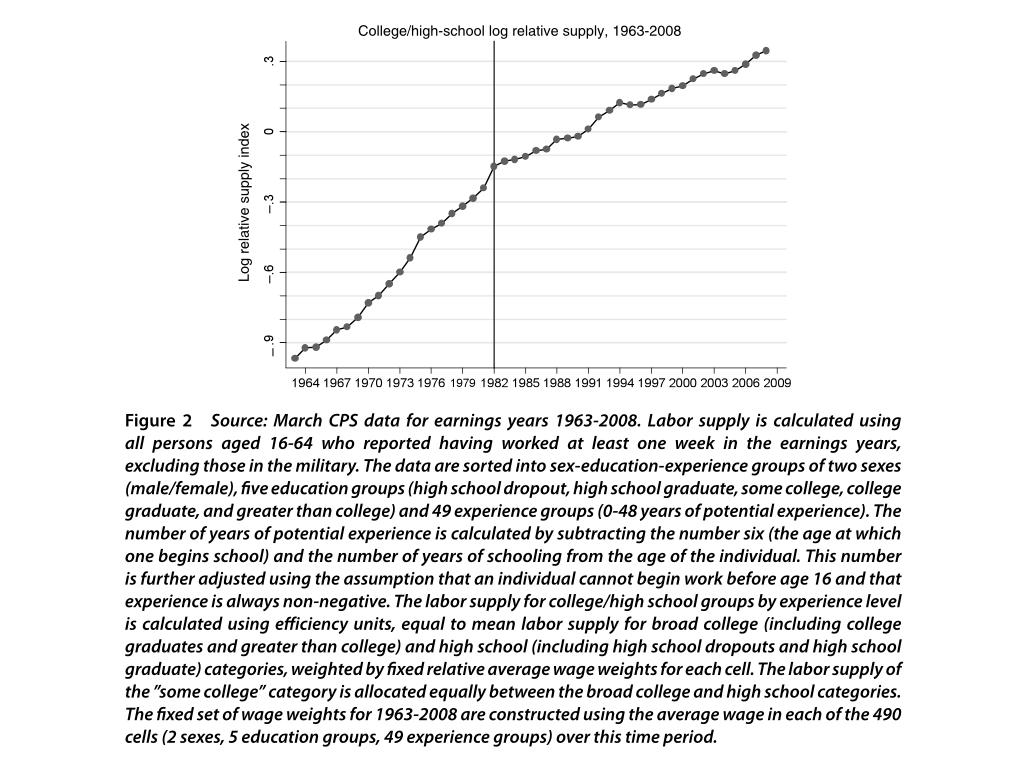
\includegraphics[height=8.5cm,width=\textwidth]{figure2.png}
\end{figure} 
\end{center}
\newpage

\newpage
\begin{center}
\begin{figure}
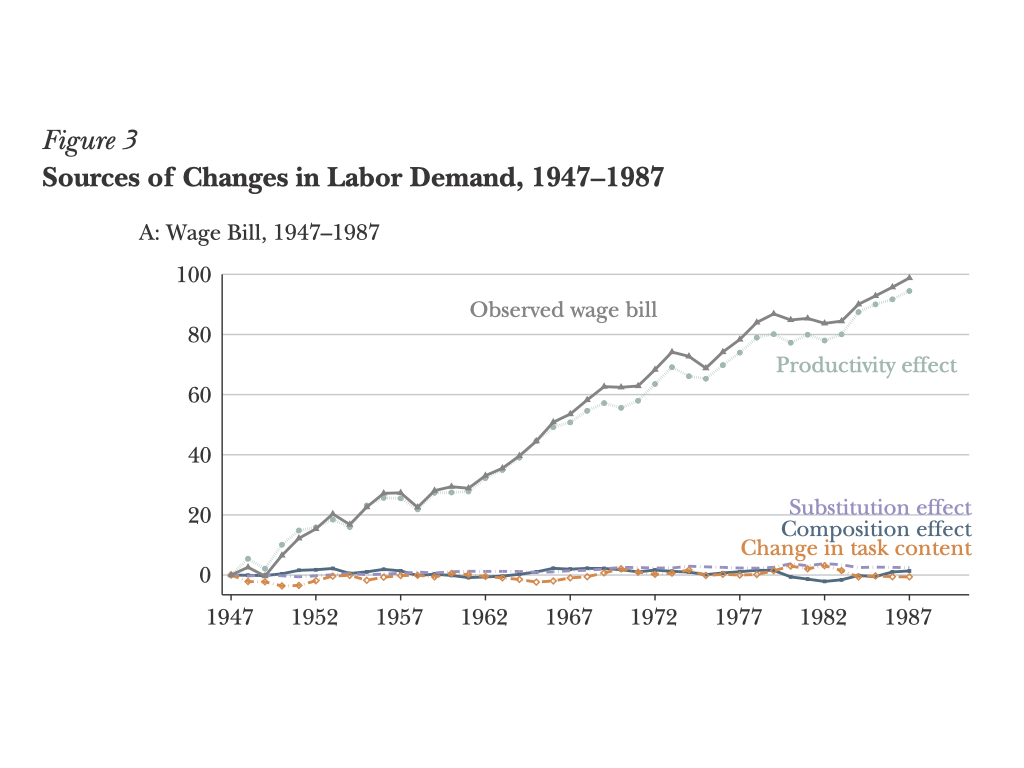
\includegraphics[height=8.5cm,width=\textwidth]{figure3a.png}
\end{figure} 
\end{center}
\newpage

\newpage
\begin{center}
\begin{figure}
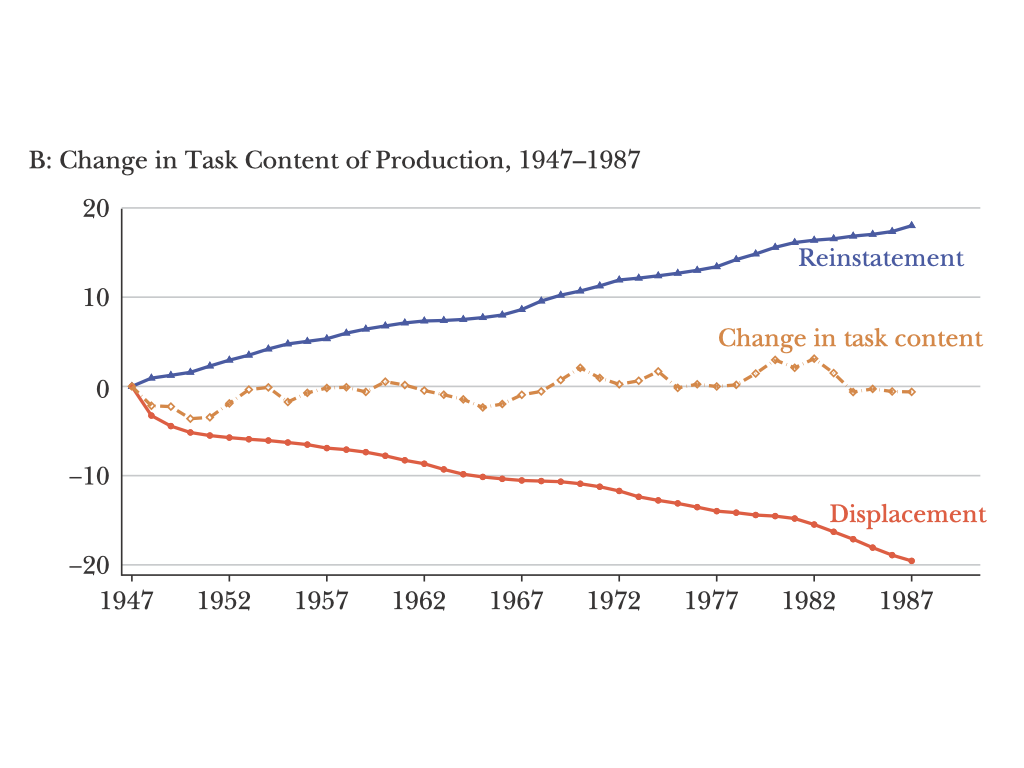
\includegraphics[height=8.5cm,width=\textwidth]{figure3b.png}
\end{figure} 
\end{center}
\newpage

\begin{frame}{Slowing growth in college attainment (Figures 2 \& 3)}
\begin{enumerate}
\item The Vietnam War boosted college attainment in the late 1960s and early 1970s to defer military service. \medskip
\item Large baby boom cohorts that entered the labor market in the 1960s and 1970s were both more educated and more numerous than existing cohorts. \medskip
\item The decline in the college premium in the 1970s (temporarly) discouraged college enrollment. \medskip
\item The male college completion rate never returned to its pre-1975 trajectory.
\end{enumerate}
\end{frame}

\subsection{2.3 Real wage levels by skill group}

\begin{frame}{2. An overview of labor market trends}
\begin{itemize}
\item[\textcolor{gray}{2.1}] \textcolor{gray}{A brief overview of data sources} \medskip
\item[\textcolor{gray}{2.2}] \textcolor{gray}{The college/high school wage premium} \medskip
\item[\textcolor{red}{2.3}] \textcolor{red}{Real wage levels by skill group} \medskip
\item[\textcolor{gray}{2.4}] \textcolor{gray}{Overall wage inequality} \medskip
\item [\textcolor{gray}{2.5}] \textcolor{gray}{Job polarization}
\end{itemize}
\end{frame}

\newpage
\begin{center}
\begin{figure}
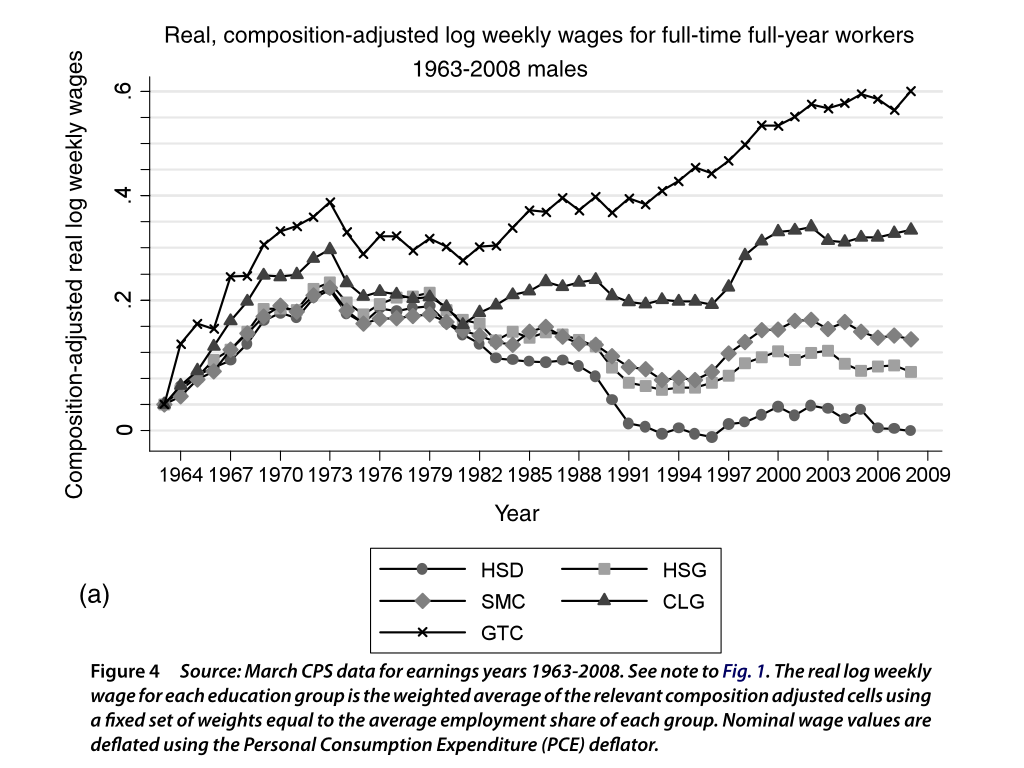
\includegraphics[height=8.5cm,width=\textwidth]{figure4a.png}
\end{figure} 
\end{center}
\newpage

\newpage
\begin{center}
\begin{figure}
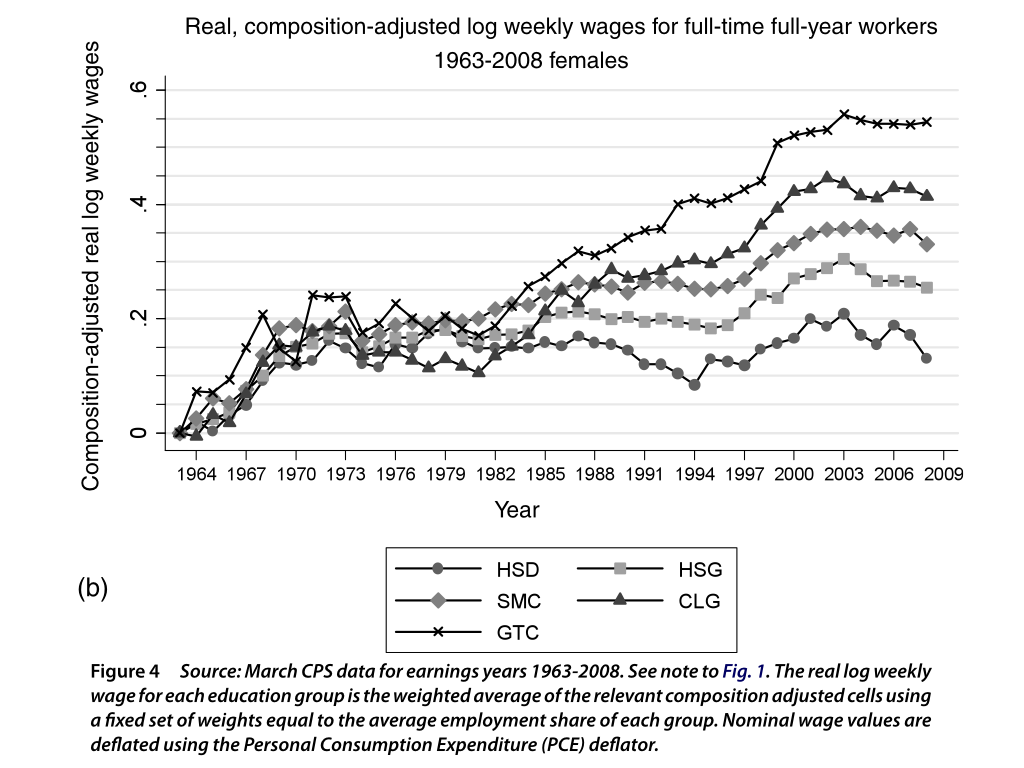
\includegraphics[height=8.5cm,width=\textwidth]{figure4b.png}
\end{figure} 
\end{center}
\newpage

\begin{frame}{Real wage levels by skill group (Figure 4)}
\begin{itemize}
\item 1963-1973: Real wages rose steeply and uniformly for both genders and all education groups. \medskip
\item 1973-1980: Wage levels stagnated for both genders and all education groups. \medskip
\item After 1980: Real wage levels of less-educated (less-experienced men) fell, whereas real wages for post-college educated rose. \medskip
\item Earnings inequality increased rapidly in the 1980s and 1990s (especially for men) and modestly in the 2000s.
\end{itemize}
\end{frame}

\newpage
\begin{center}
\begin{figure}
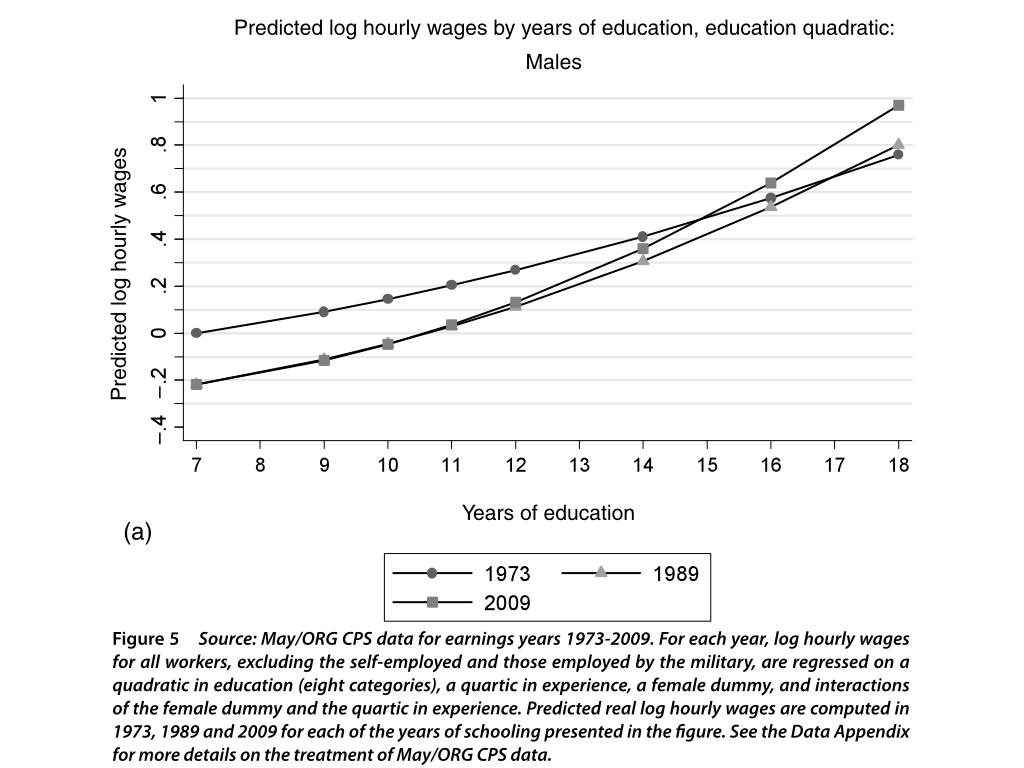
\includegraphics[height=8.5cm,width=\textwidth]{figure5a.png}
\end{figure} 
\end{center}
\newpage

\newpage
\begin{center}
\begin{figure}
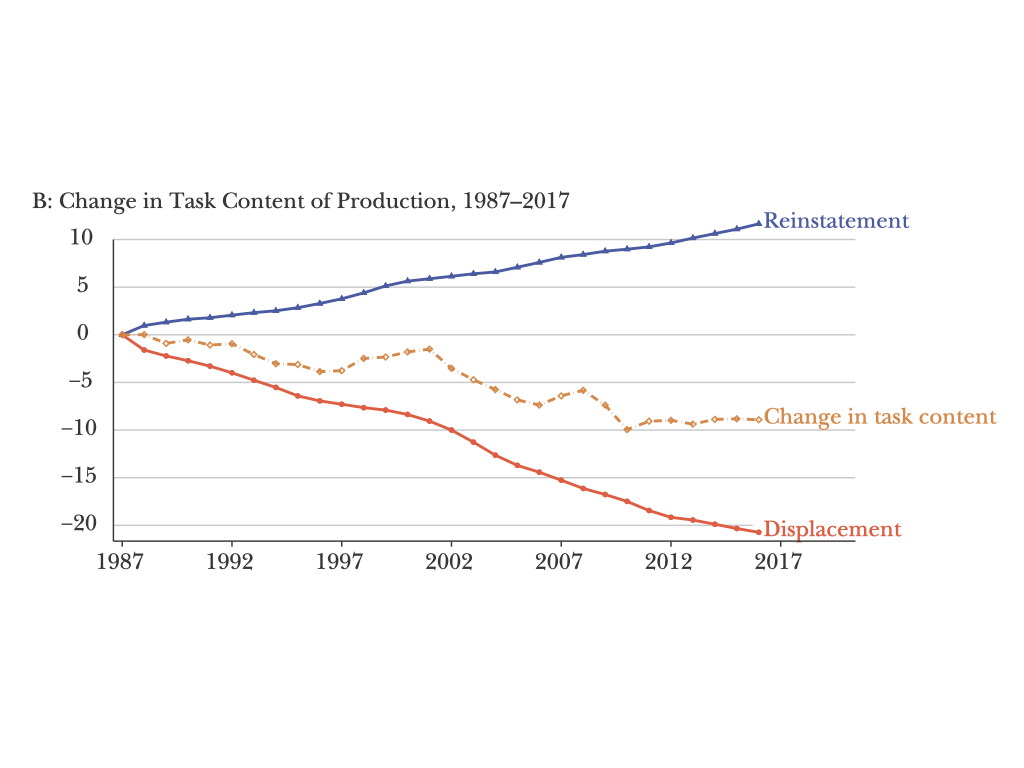
\includegraphics[height=8.5cm,width=\textwidth]{figure5b.png}
\end{figure} 
\end{center}
\newpage
\newpage
\begin{center}
\begin{figure}
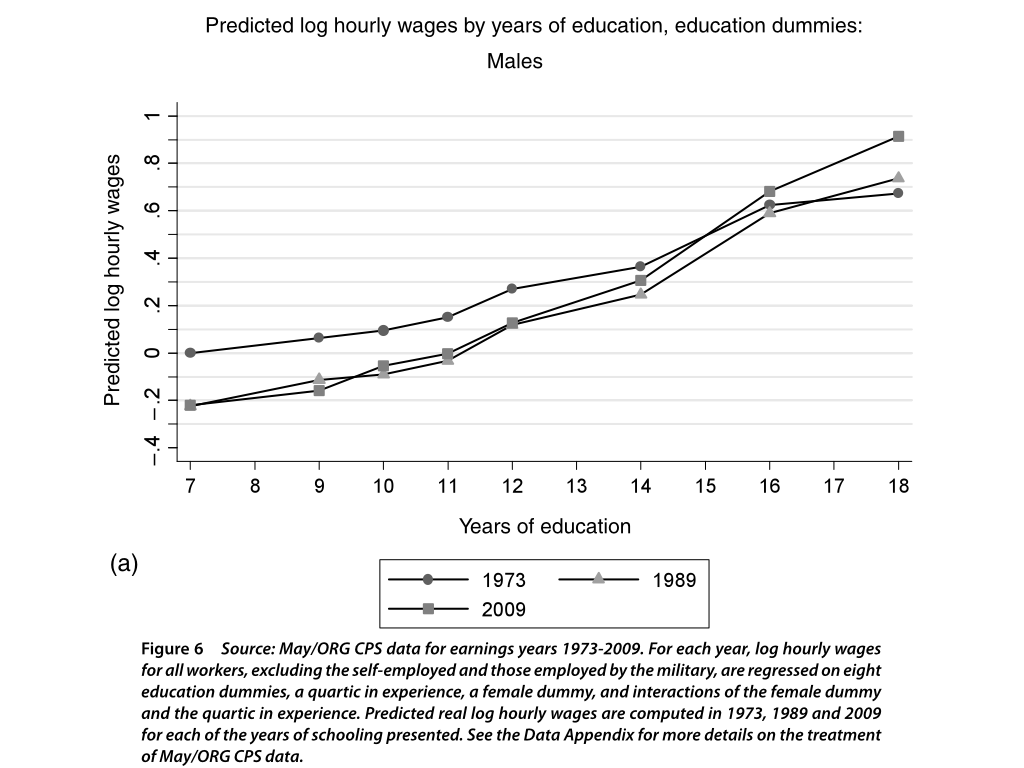
\includegraphics[height=8.5cm,width=\textwidth]{figure6a.png}
\end{figure} 
\end{center}
\newpage

\newpage
\begin{center}
\begin{figure}
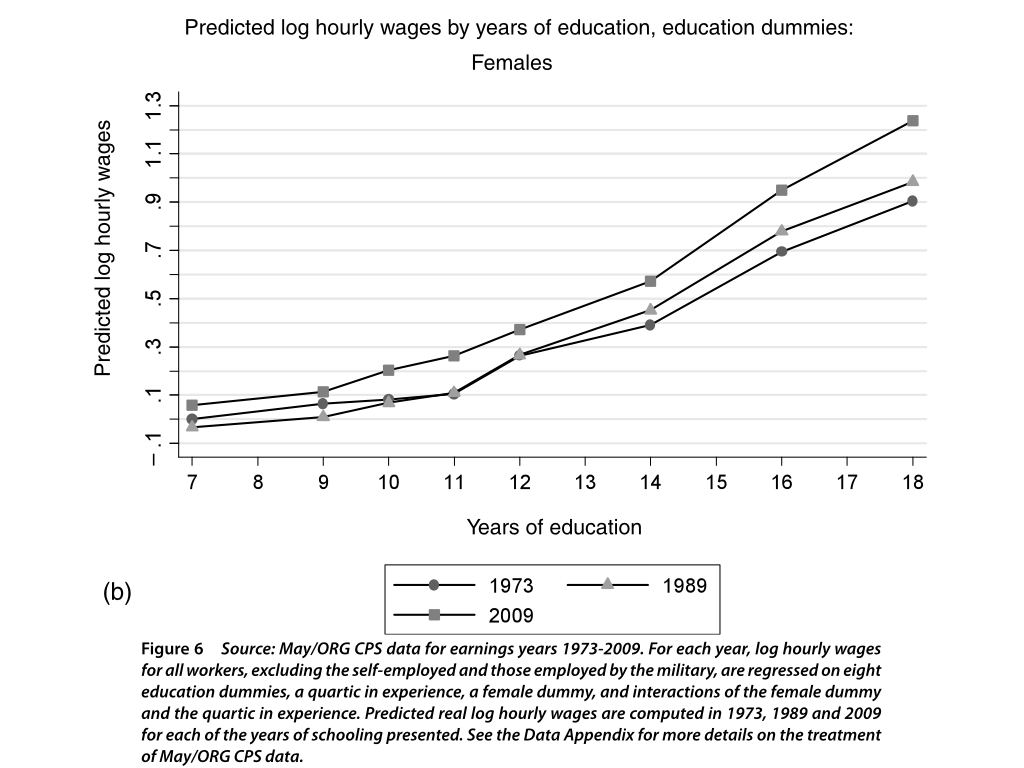
\includegraphics[height=8.5cm,width=\textwidth]{figure6b.png}
\end{figure} 
\end{center}
\newpage

\subsection{2.4 Overall wage inequality}

\begin{frame}{2. An overview of labor market trends}
\begin{itemize}
\item[\textcolor{gray}{2.1}] \textcolor{gray}{A brief overview of data sources} \medskip
\item[\textcolor{gray}{2.2}] \textcolor{gray}{The college/high school wage premium} \medskip
\item[\textcolor{gray}{2.3}] \textcolor{gray}{Real wage levels by skill group} \medskip
\item[\textcolor{red}{2.4}] \textcolor{red}{Overall wage inequality} \medskip
\item [\textcolor{gray}{2.5}] \textcolor{gray}{Job polarization}
\end{itemize}
\end{frame}

\begin{frame}{Overall wage inequality}
\begin{itemize}
\item Evolution of real and relative wages by education, gender and experience groups does not capture all changes in the wage distribution. \medskip
\item Summarize the entire earnings distribution by showing trends in real wages by percentile. \medskip
\item Focus on the 10th to 90th percentiles because CPS samples are unlikely to provide accurate measures of earnings at the highest and lowest percentiles.
\end{itemize}
\end{frame}

\newpage
\begin{center}
\begin{figure}
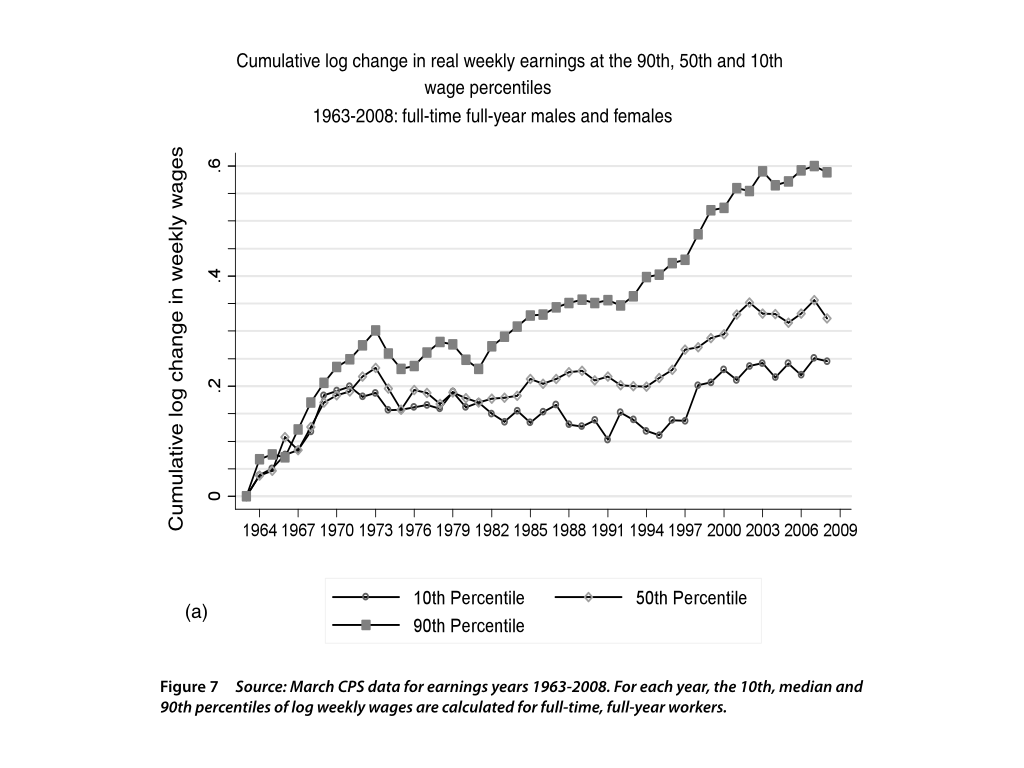
\includegraphics[height=8.5cm,width=\textwidth]{figure7a.png}
\end{figure} 
\end{center}
\newpage

\newpage
\begin{center}
\begin{figure}
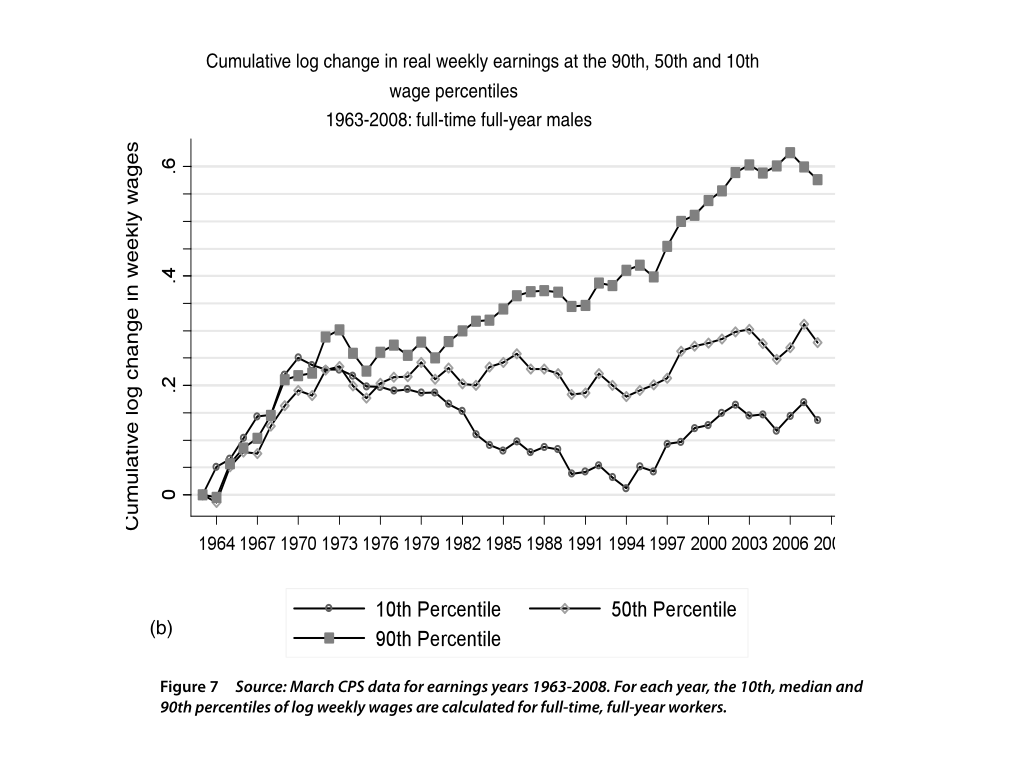
\includegraphics[height=8.5cm,width=\textwidth]{figure7b.png}
\end{figure} 
\end{center}
\newpage

\newpage
\begin{center}
\begin{figure}
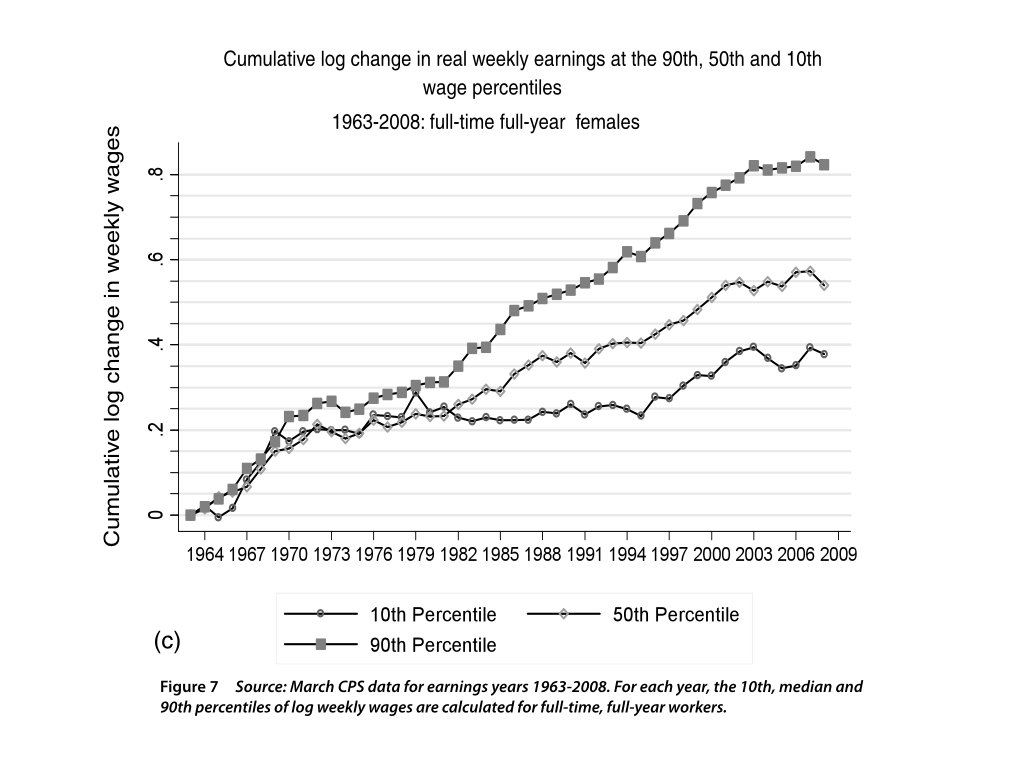
\includegraphics[height=8.5cm,width=\textwidth]{figure7c.png}
\end{figure} 
\end{center}
\newpage

\begin{frame}{Overall wage inequality (Figure 7)}
\begin{itemize}
\item 1963-1973: All percentiles rise relatively evenly. \medskip 
\item 1973-1980: Median and 10th percentile stagnate, and the 90th percentile pulls away modestly. \medskip
\item 1980-2000: Median is flat, the 10th percentile falls and the 90th percentile grows, increasing overall inequality. \medskip
\item After 2000: Median and 10th percentile grow and the 90th percentile grows faster, modestly increasing overall inequality.
\end{itemize}
\end{frame}

\newpage
\begin{center}
\begin{figure}
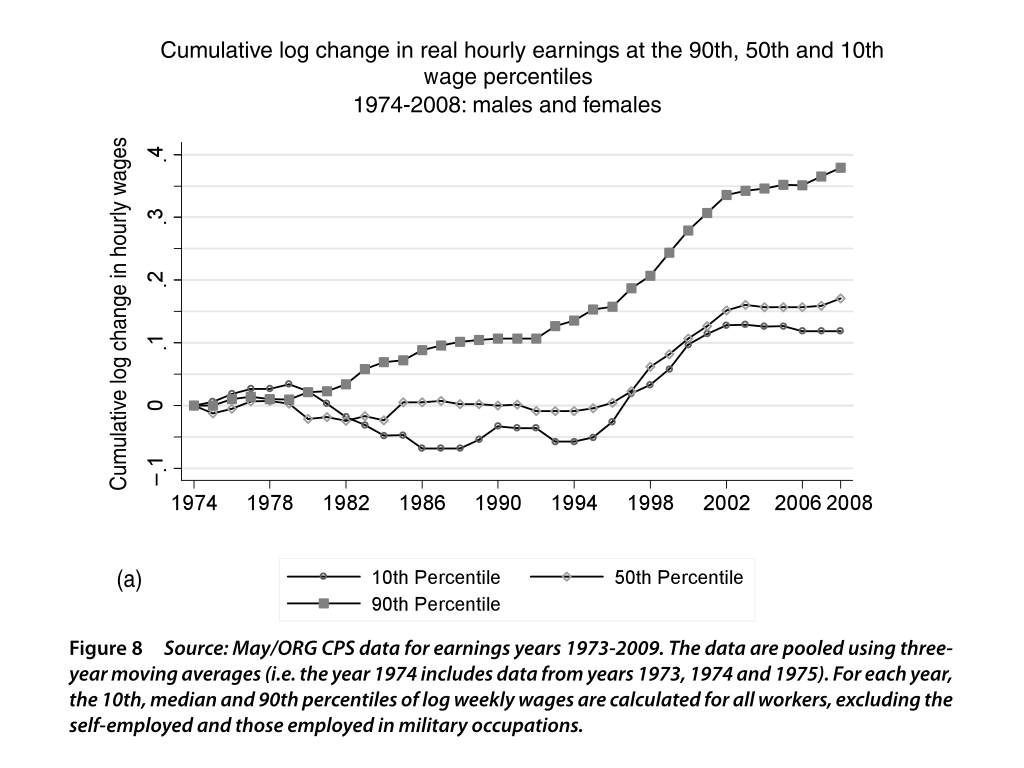
\includegraphics[height=8.5cm,width=\textwidth]{figure8a.png}
\end{figure} 
\end{center}
\newpage

\newpage
\begin{center}
\begin{figure}
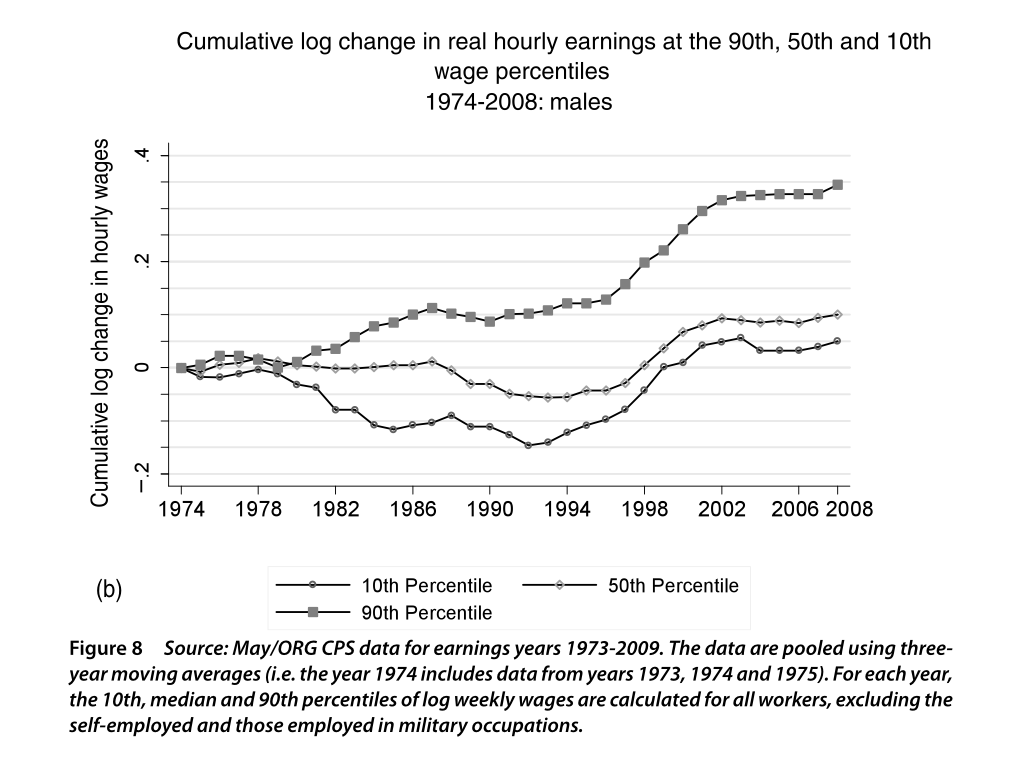
\includegraphics[height=8.5cm,width=\textwidth]{figure8b.png}
\end{figure} 
\end{center}
\newpage

\newpage
\begin{center}
\begin{figure}
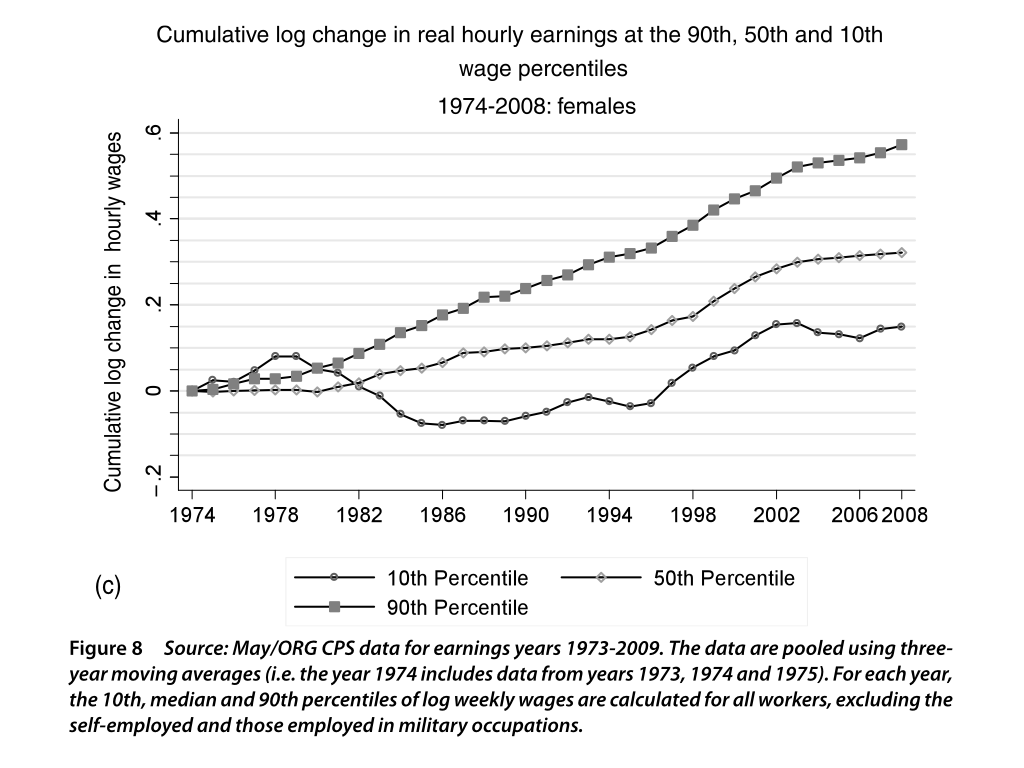
\includegraphics[height=8.5cm,width=\textwidth]{figure8c.png}
\end{figure} 
\end{center}
\newpage

\begin{frame}{Overall wage inequality (Figure 8)}
\begin{itemize}
\item Figure 7 depicted trends in average weekly wages for for FTFY workers using the March CPS. \medskip
\item Figure 8 shows trends in average hourly wages for all hourly and salary workers using the MORG CPS. \medskip
\item The evolution of the 10th percentile is much more volatile: It decreases between 1979-1988, stagnates between 1988-1995, grows rapidly between 1995-2003, and stagnates afterwards. \medskip 
\item There has been ``wage polarization'' after 1988.
\end{itemize}
\end{frame}

\newpage
\begin{center}
\begin{figure}
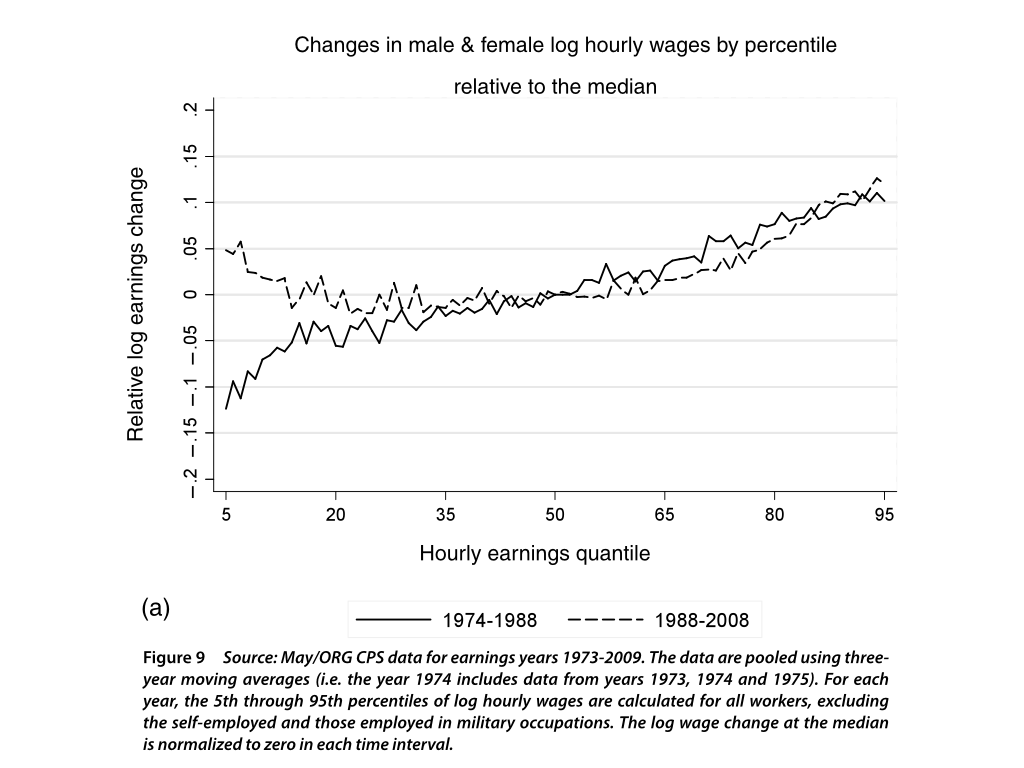
\includegraphics[height=8.5cm,width=\textwidth]{figure9a.png}
\end{figure} 
\end{center}
\newpage

\newpage
\begin{center}
\begin{figure}
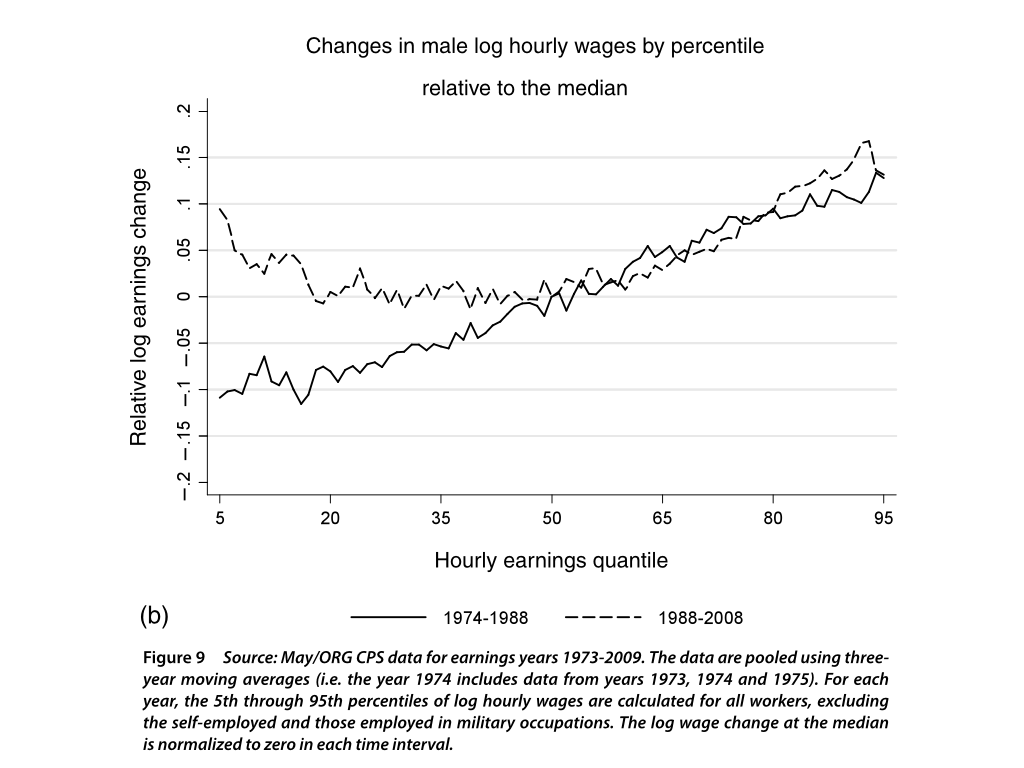
\includegraphics[height=8.5cm,width=\textwidth]{figure9b.png}
\end{figure} 
\end{center}
\newpage

\newpage
\begin{center}
\begin{figure}
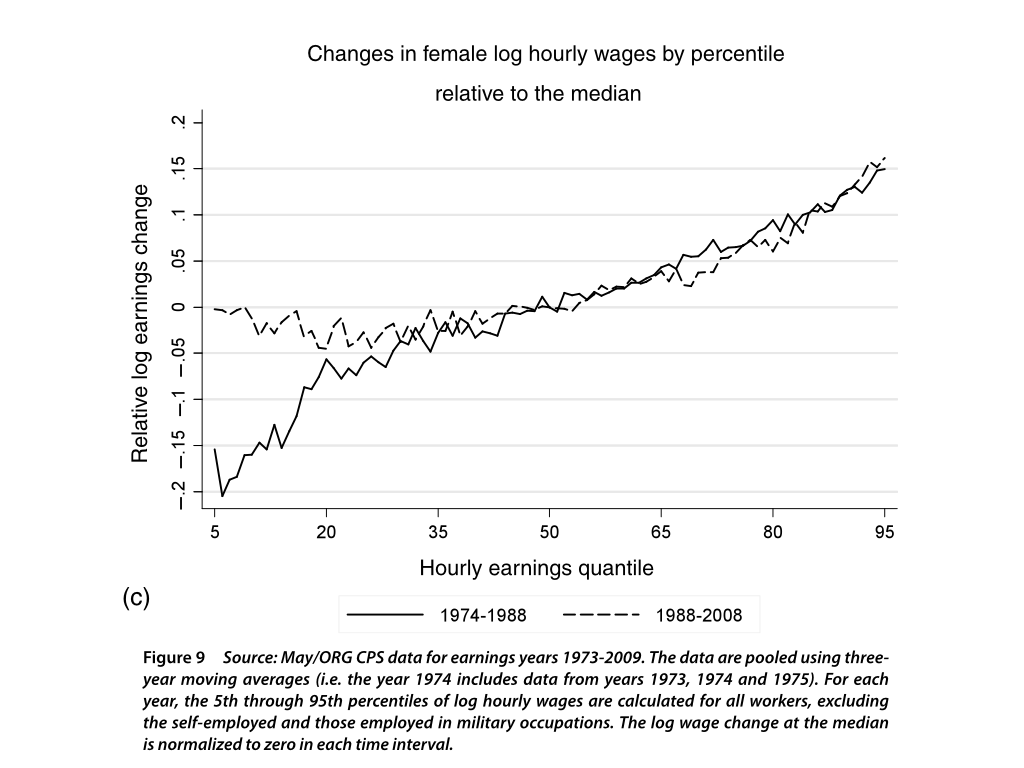
\includegraphics[height=8.5cm,width=\textwidth]{figure9c.png}
\end{figure} 
\end{center}
\newpage

\subsection{2.5 Job polarization}

\begin{frame}{2. An overview of labor market trends}
\begin{itemize}
\item[\textcolor{gray}{2.1}] \textcolor{gray}{A brief overview of data sources} \medskip
\item[\textcolor{gray}{2.2}] \textcolor{gray}{The college/high school wage premium} \medskip
\item[\textcolor{gray}{2.3}] \textcolor{gray}{Real wage levels by skill group} \medskip
\item[\textcolor{gray}{2.4}] \textcolor{gray}{Overall wage inequality} \medskip
\item [\textcolor{red}{2.5}] \textcolor{red}{Job polarization}
\end{itemize}
\end{frame}

\newpage
\begin{center}
\begin{figure}
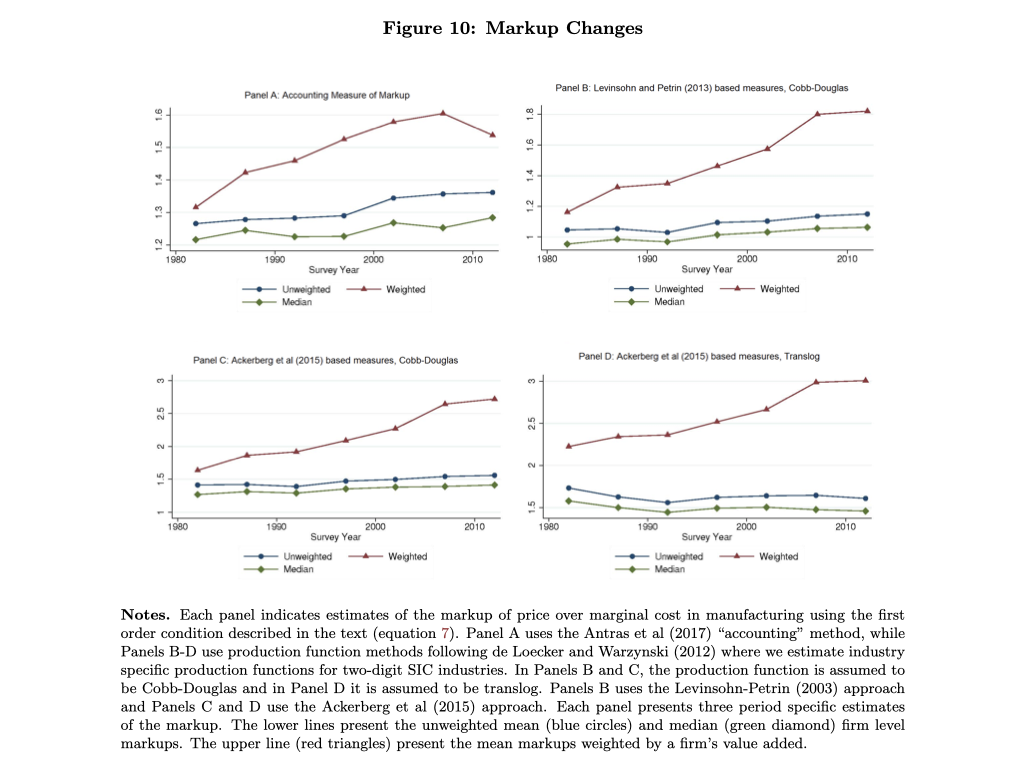
\includegraphics[height=8.5cm,width=\textwidth]{figure10.png}
\end{figure} 
\end{center}
\newpage

\newpage
\begin{center}
\begin{figure}
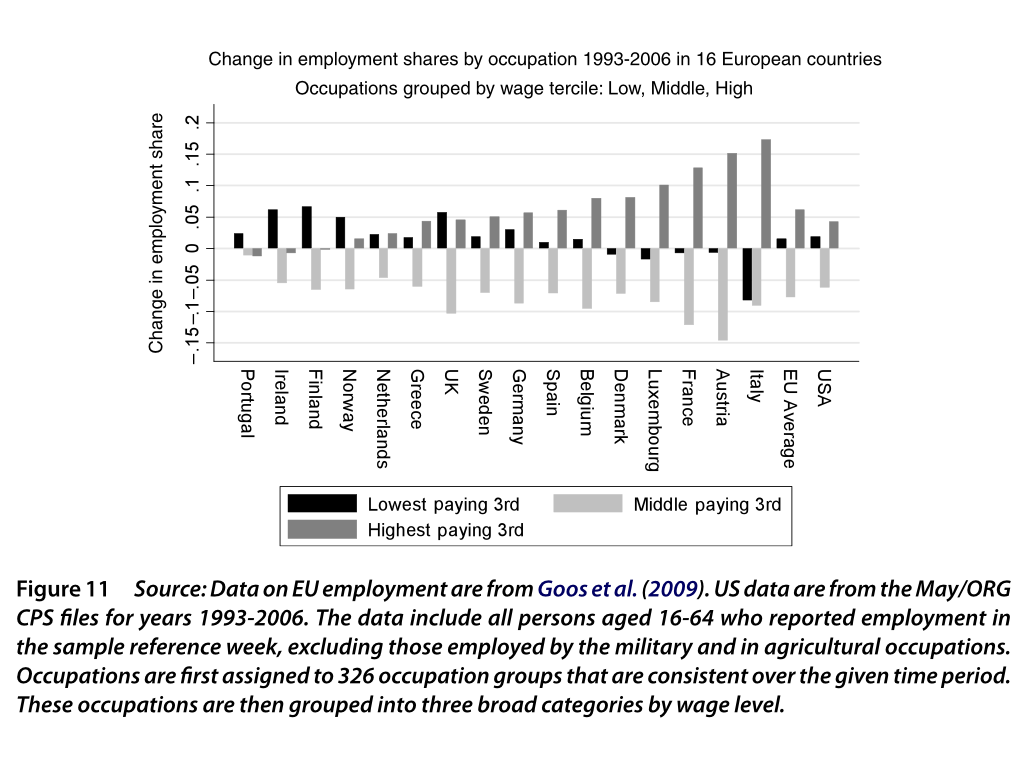
\includegraphics[height=8.5cm,width=\textwidth]{figure11.png}
\end{figure} 
\end{center}
\newpage

\newpage
\begin{center}
\begin{figure}
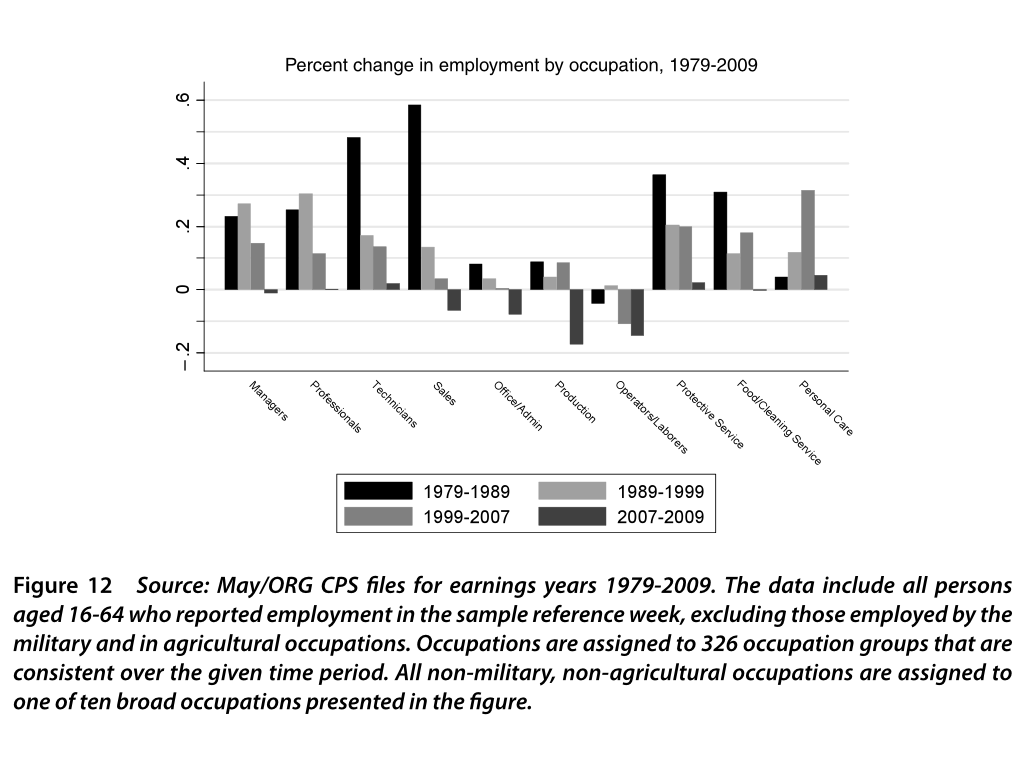
\includegraphics[height=8.5cm,width=\textwidth]{figure12.png}
\end{figure} 
\end{center}
\newpage

\newpage
\begin{center}
\begin{figure}
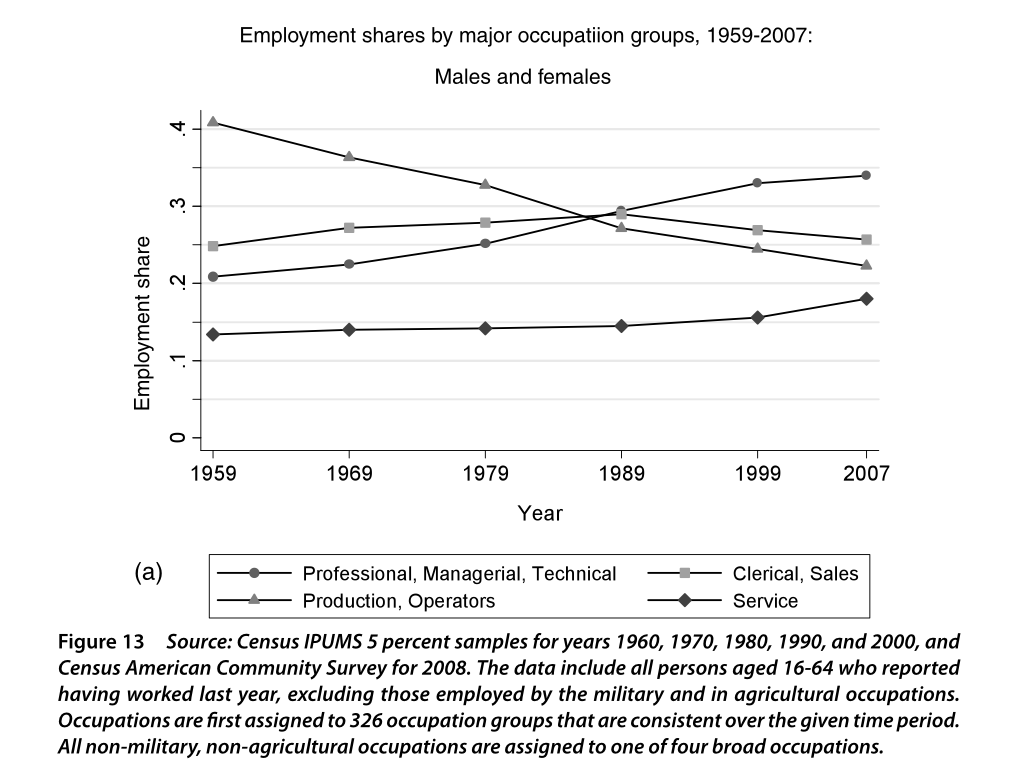
\includegraphics[height=8.5cm,width=\textwidth]{figure13a.png}
\end{figure} 
\end{center}
\newpage

\newpage
\begin{center}
\begin{figure}
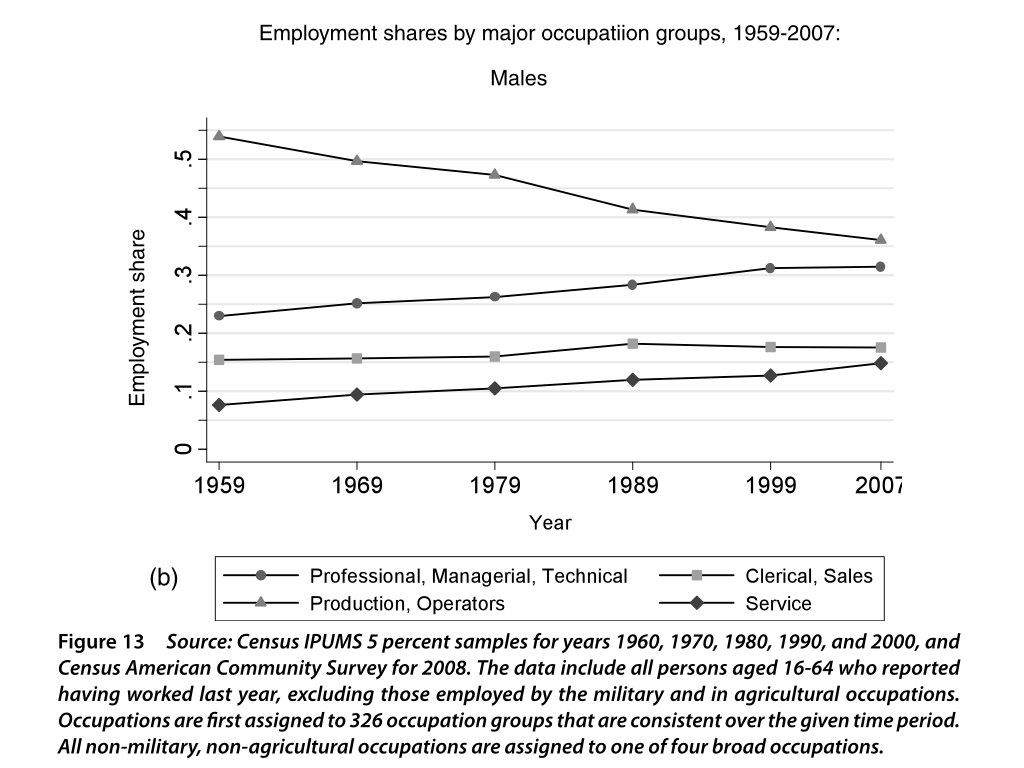
\includegraphics[height=8.5cm,width=\textwidth]{figure13b.png}
\end{figure} 
\end{center}
\newpage

\newpage
\begin{center}
\begin{figure}
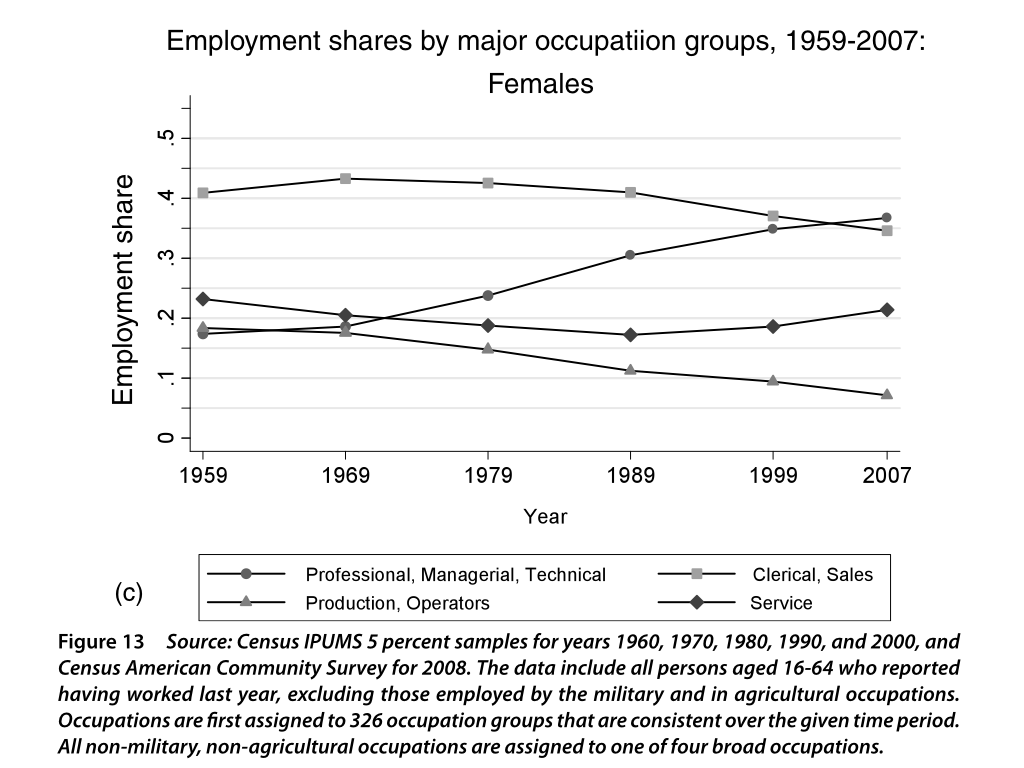
\includegraphics[height=8.5cm,width=\textwidth]{figure13c.png}
\end{figure} 
\end{center}
\newpage

\begin{frame}{Is job polarization explained by industrial composition?}
\begin{itemize}
\item The change in employment in occupation $j$ can be decomposed as:
\[
\Delta E_{jt}=\sum\nolimits_{k} \Delta E_{kt} \lambda_{jk}+\sum\nolimits_{k} \Delta \lambda _{jkt} E_{k} \tag{1} \label{eq1}
\]
with $ \Delta E_{kt}$ the change over time in employment in industry $k$; $ \lambda_{jk}$ the share of occupation $j$ in industry $k$ averaged across years; $ \Delta \lambda_{jkt}$ the change over time in the share of occupation $j$ in industry $k$; and $ E_{k}$ employment in $k$ averaged over time.\medskip
\item Within-industry shifts against middle-skilled and favoring high- and low-skilled occupations are the primary driver for job polarization.
\end{itemize}
\end{frame}

\begin{frame}{The growing importance of occupations in wages}
\begin{itemize}
\item Employment polarization combined with wage polarization suggests that workers' occupational affiliations may have become a more important determinant of wages. \medskip
\item Use Census and ACS data for 1959-2007 and regress FTFY weekly wages onto education, experience, occupation dummies, industry dummies, and task measures. \medskip
\item Calculate the partial $R^2$ (net of experience) for each set of regressors in each year for men and women separately. \medskip
\item Partial $R^2$ for occupation dummies and task measures have increased since 1979.
\end{itemize}
\end{frame}

\newpage
\begin{center}
\begin{figure}
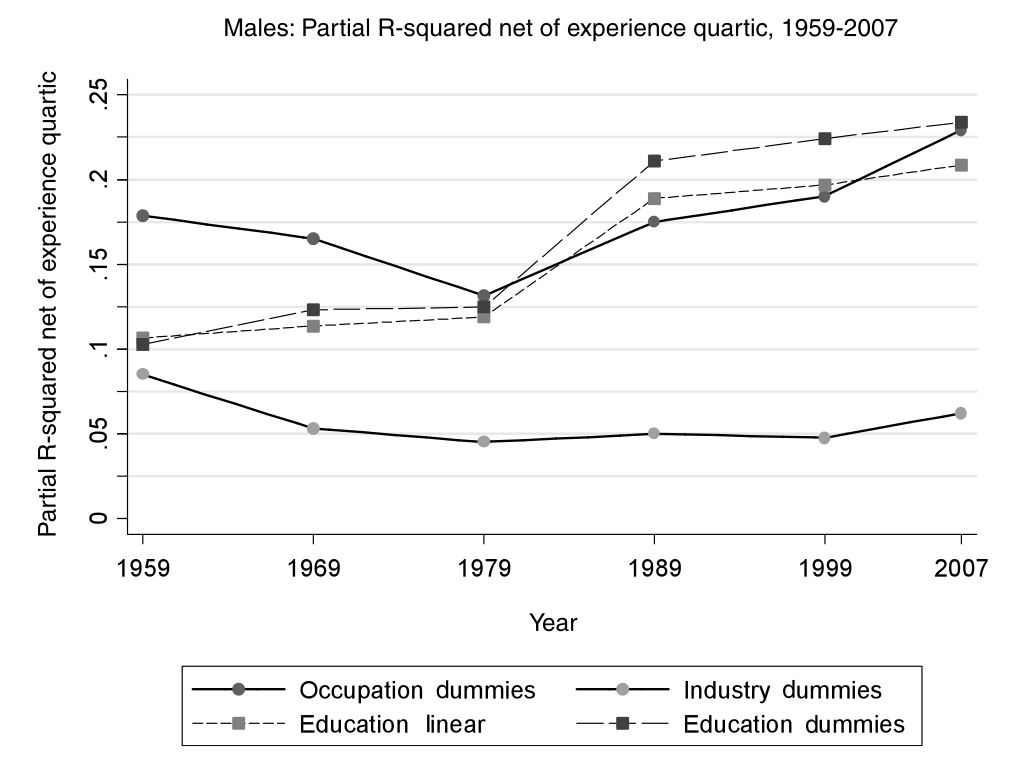
\includegraphics[height=8.5cm,width=\textwidth]{figure17a.png}
\end{figure} 
\end{center}
\newpage

\newpage
\begin{center}
\begin{figure}
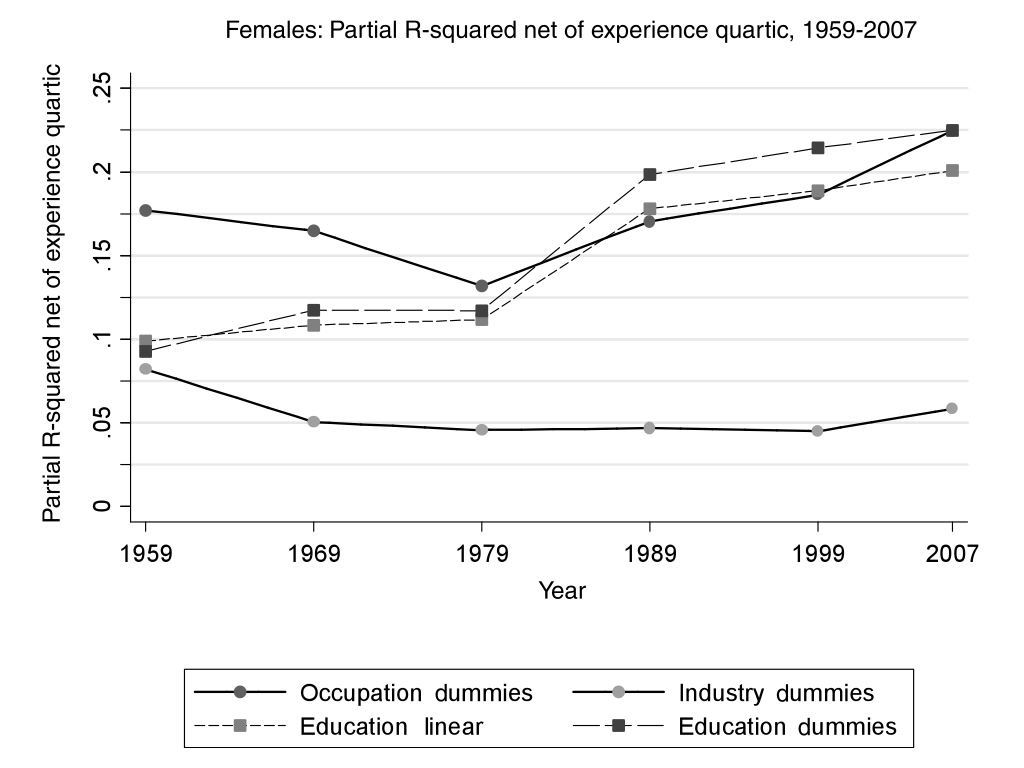
\includegraphics[height=8.5cm,width=\textwidth]{figure17b.png}
\end{figure} 
\end{center}
\newpage

\newpage
\begin{center}
\begin{figure}
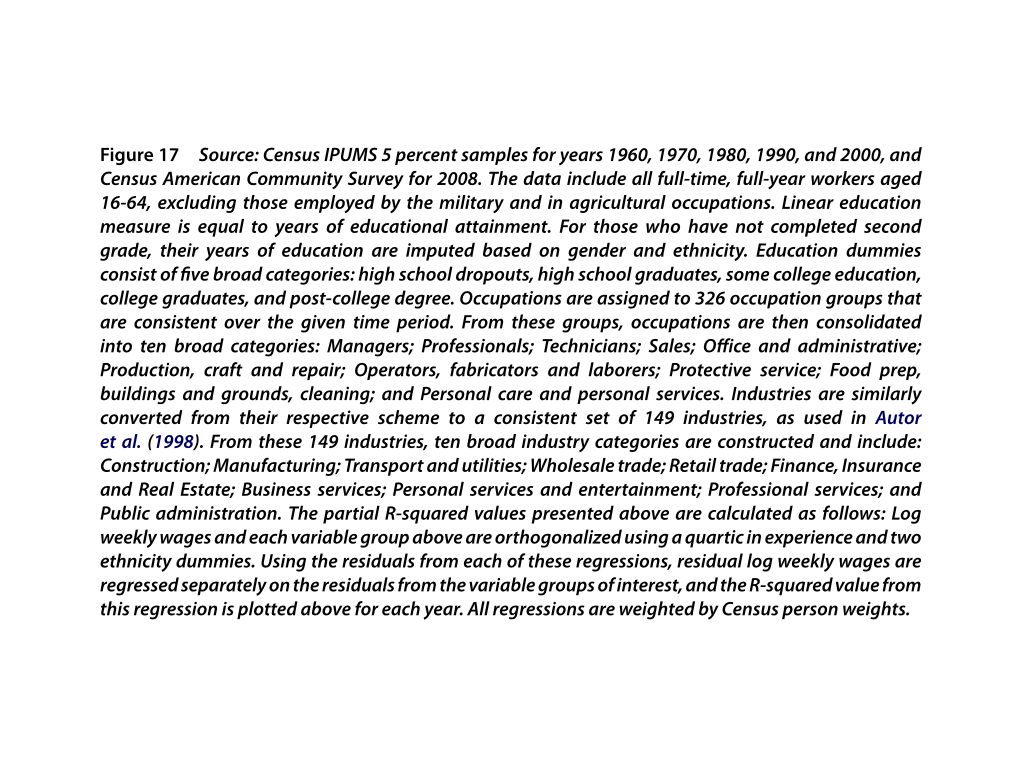
\includegraphics[height=8.5cm,width=\textwidth]{figure17notes.png}
\end{figure} 
\end{center}
\newpage

\newpage
\begin{center}
\begin{figure}
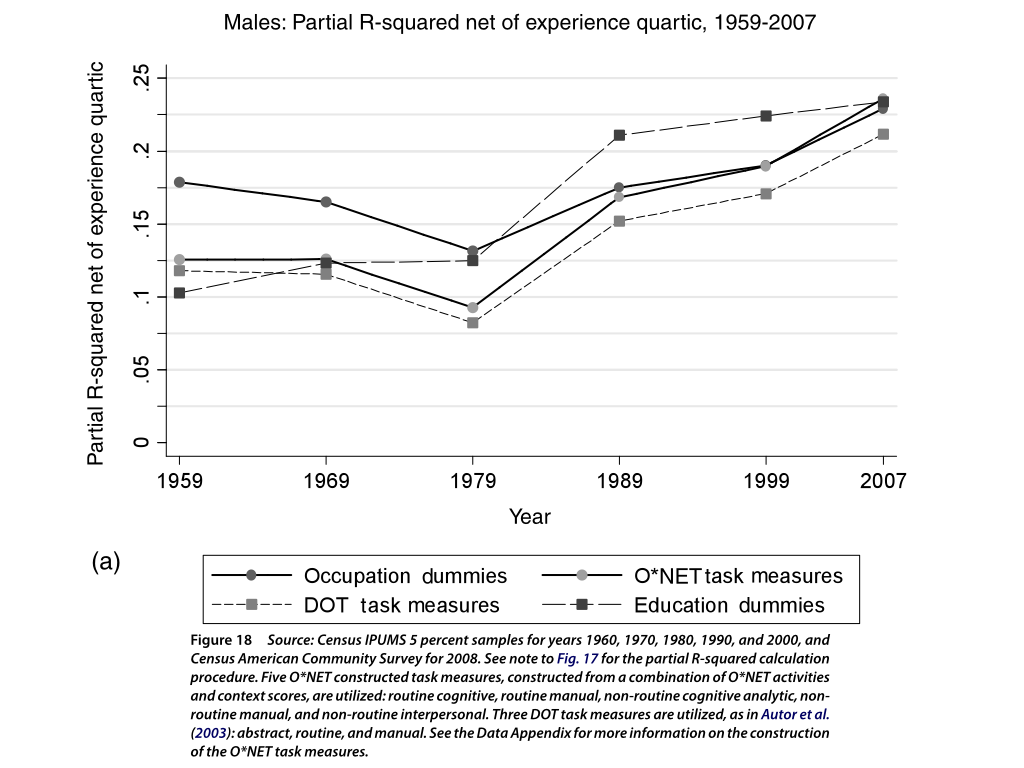
\includegraphics[height=8.5cm,width=\textwidth]{figure18a.png}
\end{figure} 
\end{center}
\newpage

\newpage
\begin{center}
\begin{figure}
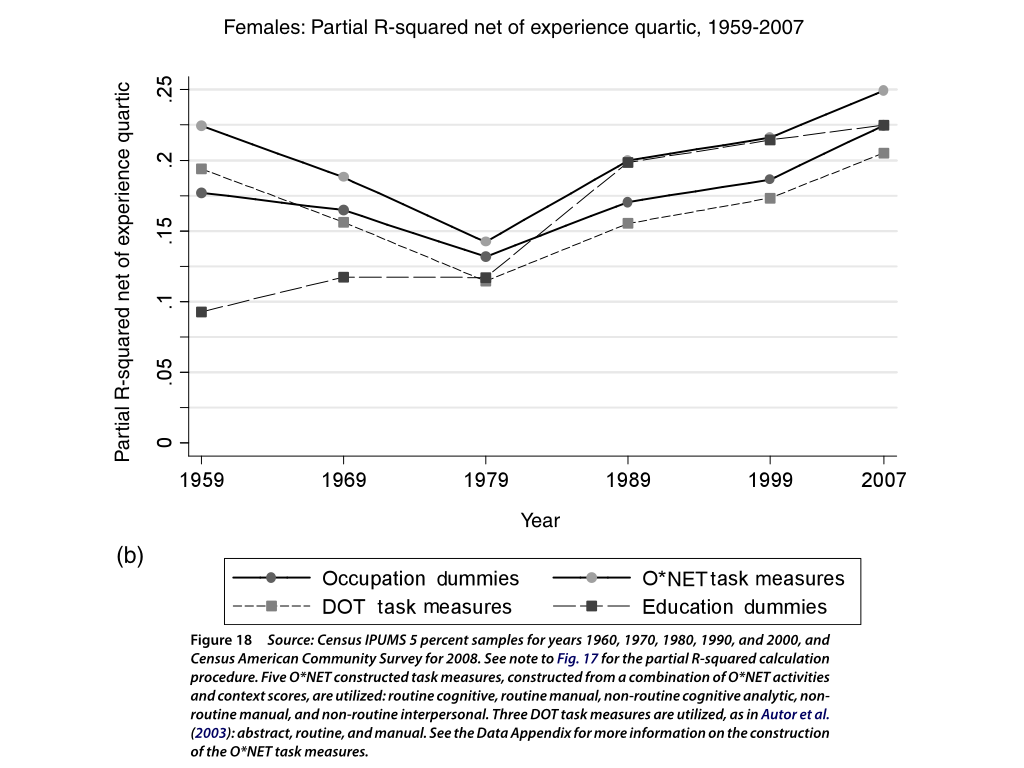
\includegraphics[height=8.5cm,width=\textwidth]{figure18b.png}
\end{figure} 
\end{center}
\newpage

\section{3. The Canonical Model}

\subsection{3.1 The simple theory of the canonical model}

\begin{frame}{3. The canonical model}
\begin{itemize}
\item[\textcolor{red}{3.1}] \textcolor{red}{The simple theory of the canonical model} \medskip
\item[\textcolor{gray}{3.2}] \textcolor{gray}{Bringing Tinbergen's education race to the data} \medskip
\item[\textcolor{gray}{3.3}] \textcolor{gray}{Changes in earnings through the lens of the canonical model} \medskip
\item[\textcolor{gray}{3.4}] \textcolor{gray}{Overall inequality in the canonical model} \medskip
\item[\textcolor{gray}{3.5}] \textcolor{gray}{Endogenous change in technology} \medskip
\item[\textcolor{gray}{3.6}] \textcolor{gray}{Summary}
\end{itemize}
\end{frame}

\begin{frame}{Tinbergen's race between education and technology}
\begin{block}{Jan Tinbergen, 1975}
\textit{``The two preponderant forces at work are technological development, which made for a relative increase in demand and hence in the income ratio... and increased access to schooling, which made for a relative decrease."}
\end{block} \medskip
Translation into the ``canonical model'': \medskip
\begin{itemize}
\item Long term trend increases towards greater relative demand and greater supply of skilled workers. \medskip
\item Bursts of supply and/or technologically-induced demand accelerations/decelerations that cause demand to temporarily move out more rapidly than supply or vice versa in some eras.
\end{itemize}
\end{frame}

\begin{frame}{CES model}
\begin{itemize}
\item Consider an aggregate CES function:
\[
Y=\left[ [A_{L}L]^{\frac{\sigma -1}{\sigma }}+[A_{H}H]^{%
\frac{\sigma -1}{\sigma }}\right] ^{\frac{\sigma }{\sigma -1}} \tag{2} \label{eq2}
\]%
with $L=\int_{i\in \mathrm{L}}l_{i}di$ and $H=\int_{i\in \mathrm{H}}h_{i}di$
where $l_{i}$ ($h_{i}$) denotes the supply in efficiency units of low (high)
educated labor that worker $i$ possesses and with $\sigma \in [0, \infty) $ the elasticiticy of substitution between $L$ and $H$.\bigskip
\item Changes in $H/L$ will capture changes in the relative supply of educated labor, whereas all other changes will capture changes in the relative demand for educated labor.
\end{itemize}
\end{frame}

\begin{frame}{Interpretations of the CES model}
\begin{enumerate}
\item Only one good, skilled and unskilled workers are imperfect substitutes in its production. \medskip
\item Two-good economy: \medskip
\begin{itemize}
\item Consumers have CES utility with elasticity of substitution in consumption of $ \sigma $ \medskip
\item Good $ Y_{L} $ is produced with $ Y_{L} = A_{L}L $ \medskip
\item Good $ Y_{H} $ is produced with $ Y_{H} = A_{H}H $ \medskip
\end{itemize}
\item A mixture of these two where different sectors produce goods that are imperfect substitutes, and low and high skilled workers are employed in all sectors.
\end{enumerate}
\end{frame}

\begin{frame}{Interpretations of $\sigma $}
\begin{itemize}
\item The CES model is an abstraction. \medskip
\item $ \sigma $ combines substitution in production and consumption across firms, industries, consumers,... \medskip
\item Surprising degree of consensus that $ \sigma \in [1,2]$ \medskip
\item When examining the impact of technological progress, we assume that $ \sigma $ captures the elasticity of substitution between input factors in an aggregate production function.
\end{itemize}
\end{frame}

\begin{frame}{Technological change in the CES model}
\begin{itemize}
\item Consider a more general aggregate CES production function:
\[
Y=\Pi \left[ \Gamma [A_{L}L + B_{L}]^{\frac{\sigma -1}{\sigma }}+[1-\Gamma][A_{H}H + B_{H}]^{%
\frac{\sigma -1}{\sigma }}\right] ^{\frac{ \sigma }{\sigma -1}} 
\]
\item Sources of technological change are: \smallskip
\begin{enumerate}
\item $A_{L}$ and $A_{H}$: Augmenting the productivity of factors (``intensive'' margin technological change). \smallskip
\item $ \Gamma $: The distribution parameter reallocates production across factors (``extensive'' margin technological change). \smallskip
\item $ \Pi $: Hicks-neutral TFP.  \smallskip
\item $ B_{L} $ and $ B_{H} $: Directly labor-replacing technologies. 
\end{enumerate}
\end{itemize}
\end{frame}

\begin{frame}{Wage setting}
\begin{itemize}
\item Assume that technological change is only factor-augmenting and skill-biased, $A_{H}/A_{L} \uparrow$ or SBTC. \medskip
\item Given the aggregate CES production function:
\[
Y=\left[ [A_{L}L]^{\frac{\sigma -1}{\sigma }} + [A_{H}H]^{%
\frac{\sigma -1}{\sigma }}\right] ^{\frac{\sigma }{\sigma -1}} \tag{2} \label{eq2}
\]
\item In equilibrium, productive efficiency implies:
\[
w_{L}=\frac{\partial Y}{\partial L}=A_{L}^{\frac{\sigma - 1}{\sigma }} \left[ A_{L}^{\frac{\sigma - 1}{\sigma}} + A_{H}^{\frac{\sigma - 1}{\sigma}} [H/L]^{\frac{\sigma - 1}{\sigma}} \right] ^{\frac{1}{\sigma - 1}} \tag{3} \label{eq3}
\]
\[
w_{H}=\frac{\partial Y}{\partial H}=A_{H}^{\frac{\sigma - 1}{\sigma }} \left[ A_{L}^{\frac{\sigma - 1}{\sigma}} [H/L]^{-\frac{\sigma - 1}{\sigma}} + A_{H}^{\frac{\sigma - 1}{\sigma}}  \right] ^{\frac{1}{\sigma - 1}} \tag{4} \label{eq4}
\]
\end{itemize}
\end{frame}

\begin{frame}{Comparative statics for low-skilled wages}
\begin{itemize}
\item We had that:
\[
w_{L}=\frac{\partial Y}{\partial L}=A_{L}^{\frac{\sigma - 1}{\sigma }} \left[ A_{L}^{\frac{\sigma - 1}{\sigma}} + A_{H}^{\frac{\sigma - 1}{\sigma}} [H/L]^{\frac{\sigma - 1}{\sigma}} \right] ^{\frac{1}{\sigma - 1}} \tag{3} \label{eq3}
\]
\item This implies the following comparative statics: \medskip
\begin{enumerate}
\item $\frac{\partial w_{L}}{\partial L} < 0$ because of decreasing marginal productivity in $L$ \medskip
\item $\frac{\partial w_{L}}{\partial H} > 0$ because of q-complementarity \medskip
\item $\frac{\partial w_{L}}{\partial A_{L}} > 0 \Leftarrow \sigma \geqslant 1 $ ($\Leftrightarrow \sigma > 1 - s_{L} $ with $s_{L}$ wagebillshare of $L$) \medskip 
\item $\frac{\partial w_{L}}{\partial A_{H}} > 0$ because of q-complementarity
\end{enumerate}
\end{itemize}
\end{frame}

\begin{frame}{Comparative statics for high-skilled wages}
\begin{itemize}
\item We had that:
\[
w_{H}=\frac{\partial Y}{\partial H}=A_{H}^{\frac{\sigma - 1}{\sigma }} \left[ A_{L}^{\frac{\sigma - 1}{\sigma}} [H/L]^{-\frac{\sigma - 1}{\sigma}} + A_{H}^{\frac{\sigma - 1}{\sigma}}  \right] ^{\frac{1}{\sigma - 1}} \tag{4} \label{eq4}
\]
\item This implies the following comparative statics: \medskip
\begin{enumerate}
\item $\frac{\partial w_{H}}{\partial H} < 0$ because of decreasing marginal productivity in $H$ \medskip
\item $\frac{\partial w_{H}}{\partial L} > 0$ because of q-complementarity \medskip
\item $\frac{\partial w_{H}}{\partial A_{H}} > 0 \Leftarrow \sigma \geqslant 1 $ ($ \Leftrightarrow \sigma > 1 - s_{H} = s_{L}$) \medskip
\item $\frac{\partial w_{H}}{\partial A_{L}} > 0$ because of q-complementarity
\end{enumerate}
\end{itemize}
\end{frame}

\begin{frame}{The skill premium}
\begin{itemize}
\item Combining (3) and (4), the skill premium is given by:
\[
\omega \equiv \frac{w_{H}}{w_{L}} = \left[ \frac{A_{H}}{A_{L}} \right] ^{ \frac{ \sigma -1}{ \sigma}}  \left[ \frac{H}{L} \right] ^ {-\frac{1}{ \sigma}} \tag{5} \label{eq5}
\]
\item Rewriting by taking logs gives:
\[
\ln( \omega ) = \frac{ \sigma - 1}{ \sigma} \ln \left( \frac{A_{H}}{A_{L}} \right) - \frac{1}{ \sigma} \ln \left( \frac{H}{L} \right)  
 \tag{6} \label{eq6}
\]
where the first term captures the first force in Tinbergen's race (i.e. technology) and the second term captures the second force (i.e. education).
\end{itemize}
\end{frame}

\begin{frame}{Comparative statics for the skill premium}
\begin{itemize}
\item We had that the skill premium is given by:
\[
\ln( \omega ) = \frac{ \sigma - 1}{ \sigma} \ln \left( \frac{A_{H}}{A_{L}} \right) - \frac{1}{ \sigma} \ln \left( \frac{H}{L} \right)  
 \tag{6} \label{eq6}
\]
\item Equation (6) implies the following comparative statics:
\[
\frac{\partial \ln( \omega )}{ \partial \ln(H/L)} = - \frac{1}{ \sigma} <0
 \tag{7} \label{eq7}
\]
\[
\frac{\partial \ln( \omega )}{ \partial \ln(A_{H}/A_{L})} = \frac{ \sigma - 1 }{ \sigma} \gtrless 0 \text{ if } \sigma \gtrless 1
 \tag{8} \label{eq8}
\]
\end{itemize}
\end{frame}

\begin{frame}{The skill premium and skill supplies}
\begin{itemize}
\item We had the comparative static:
\[
\frac{\partial \ln( \omega )}{ \partial \ln(H/L)} = - \frac{1}{ \sigma} <0
 \tag{7} \label{eq7}
\]
\item There are 2 types of substitution depending on how you interprete the CES model: \medskip
\begin{enumerate}
\item $H$ and $L$ are used to produce the same good and an increase in $H/L$ reduces the marginal productivity of  $H$ relative to $L$ and hence its relative wage.  \medskip
\item $H$ and $L$ are producing different goods and an increase in $H/L$ reduces the marginal utility of consumption of $H$ relative to $L$ and hence the its real price and relative wage.
\end{enumerate}
\end{itemize}
\end{frame}

\begin{frame}{The skill premium and SBTC}
\begin{itemize}
\item We had the comparative static:
\[
\frac{\partial \ln( \omega )}{ \partial \ln(A_{H}/A_{L})} = \frac{ \sigma - 1 }{ \sigma} \gtrless 0 \text{ if } \sigma \gtrless 1
 \tag{8} \label{eq8}
\]
\item What happens to the skill premium depends on $ \sigma \gtrless 1 $: \bigskip
\begin{enumerate}
\item \underline{If $ \sigma > 1 $}: Despite an increase in $A_{H}/A_{L}$, \textit{relative} demand for $H/L$ increases because there is enough substitution towards $H$.\bigskip
\item \underline{If $ \sigma = 1 $}: The skill premium doesn't change. \bigskip
\item \underline{If $ \sigma < 1 $}: Because of an increase in $A_{H}/A_{L}$ and limited substitution towards $H$, \textit{relative} demand for $H/L$ decreases.
\end{enumerate}
\end{itemize}
\end{frame}

\begin{frame}{Summary of key relationships}
\underline{An increase in $H$} holding $L$, $A_{H}$ and $A_{L}$ constant: \medskip
\begin{enumerate}
\item Skilled workers: $w_{H} \downarrow $ (decreasing marginal product). \medskip
\item Unskilled workers: $ w_{L} \uparrow $ (q-complementarity) \medskip
\item Skill premium: $ \omega \equiv w_{H}/w_{L} \downarrow $ \medskip
\end{enumerate}
\underline{An increase in $A_{H}$} holding $A_{L}$, $H$ and $L$ constant: \medskip
\begin{enumerate}
\item Skilled workers: $w_{H} \uparrow \Leftarrow \sigma \geqslant 1 $ ($\Leftrightarrow \sigma > 1 - s_{H} = s_{L} $) \medskip
\item Unskilled workers: $ w_{L} \uparrow $ (q-complementarity)\medskip
\item Skill premium: $ \omega \equiv w_{H}/w_{L} \gtrless 0 $ if $ \sigma \gtrless 1 $ \medskip
\end{enumerate}
\end{frame}

\subsection{3.2 Bringing Tinbergen's education race to the data}

\begin{frame}{3. The canonical model}
\begin{itemize}
\item[\textcolor{gray}{3.1}] \textcolor{gray}{The simple theory of the canonical model} \medskip
\item[\textcolor{red}{3.2}] \textcolor{red}{Bringing Tinbergen's education race to the data} \medskip
\item[\textcolor{gray}{3.3}] \textcolor{gray}{Changes in earnings through the lens of the canonical model} \medskip
\item[\textcolor{gray}{3.4}] \textcolor{gray}{Overall inequality in the canonical model} \medskip
\item[\textcolor{gray}{3.5}] \textcolor{gray}{Endogenous change in technology} \medskip
\item[\textcolor{gray}{3.6}] \textcolor{gray}{Summary}
\end{itemize}
\end{frame}

\begin{frame}{Bringing Tinbergen's education race to the data}
\begin{itemize}
\item Assume that SBTC is log linear in demand for skills:
\[
\ln (\frac{A_{Ht}}{A_{Lt}})=\gamma _{0}+\gamma _{1}t \text{ with } \gamma_{1} > 0 \tag{9}  \label{eq9}
\]
\item Substituting into equation (6) gives:
\[
\ln ( \omega_{t})=\frac{\sigma -1}{\sigma} \gamma _{0}+\frac{\sigma -1}{\sigma}\gamma _{1}t-\frac{1}{\sigma }\ln (\frac{H_{t}}{L_{t}})  \tag{10}  \label{eq10}
\]
\item Assuming that $ \sigma >1$, the skill premium will increase if SBTC exceeds the growth in education.
\end{itemize}
\end{frame}

\subsection{3.3 Changes in earnings through the lens of the canonical model}

\begin{frame}{3. The canonical model}
\begin{itemize}
\item[\textcolor{gray}{3.1}] \textcolor{gray}{The simple theory of the canonical model} \medskip
\item[\textcolor{gray}{3.2}] \textcolor{gray}{Bringing Tinbergen's education race to the data} \medskip
\item[\textcolor{red}{3.3}] \textcolor{red}{Changes in earnings through the lens of the canonical model} \medskip
\item[\textcolor{gray}{3.4}] \textcolor{gray}{Overall inequality in the canonical model} \medskip
\item[\textcolor{gray}{3.5}] \textcolor{gray}{Endogenous change in technology} \medskip
\item[\textcolor{gray}{3.6}] \textcolor{gray}{Summary}
\end{itemize}
\end{frame}

\begin{frame}{An update of Katz \& Murphy [92]}
\begin{itemize}
\item Katz \& Murphy [92] formalized Tinbergen's race between education and technology. \medskip
\item They introduced the ``canonical model'' and ``SBTC''. \medskip
\item For the period 1963-1987, Katz \& Murphy [92] estimate:
\[
\ln(\frac{w_{Ht}}{w_{Lt}})  = \beta_{0} + \beta_{1} \ln(\frac{H_{t}}{L_{t}}) + \beta_{2} t + \epsilon_{t} 
\]
\item Consider the period 1963-1987 as in Katz \& Murphy [92]. \medskip
\item Make out of sample predictions for the period 1987-2008.
\end{itemize}
\end{frame}

\newpage
\begin{center}
\begin{figure}
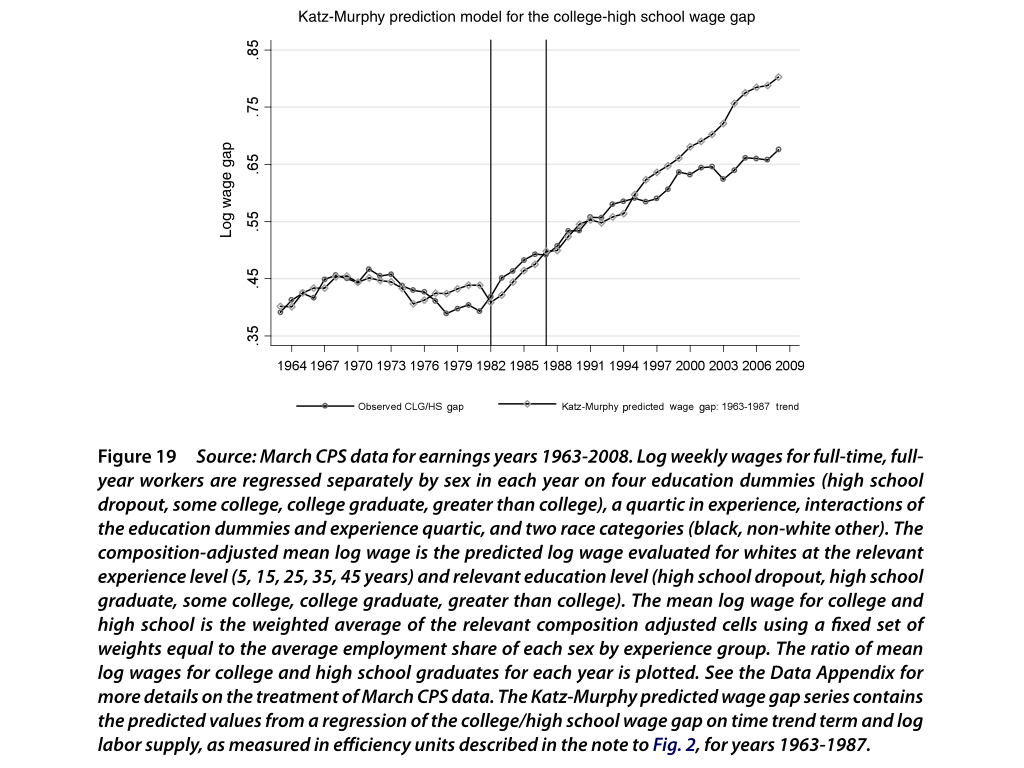
\includegraphics[height=8.5cm,width=\textwidth]{figure19.png}
\end{figure} 
\end{center}
\newpage

\newpage
\begin{center}
\begin{figure}
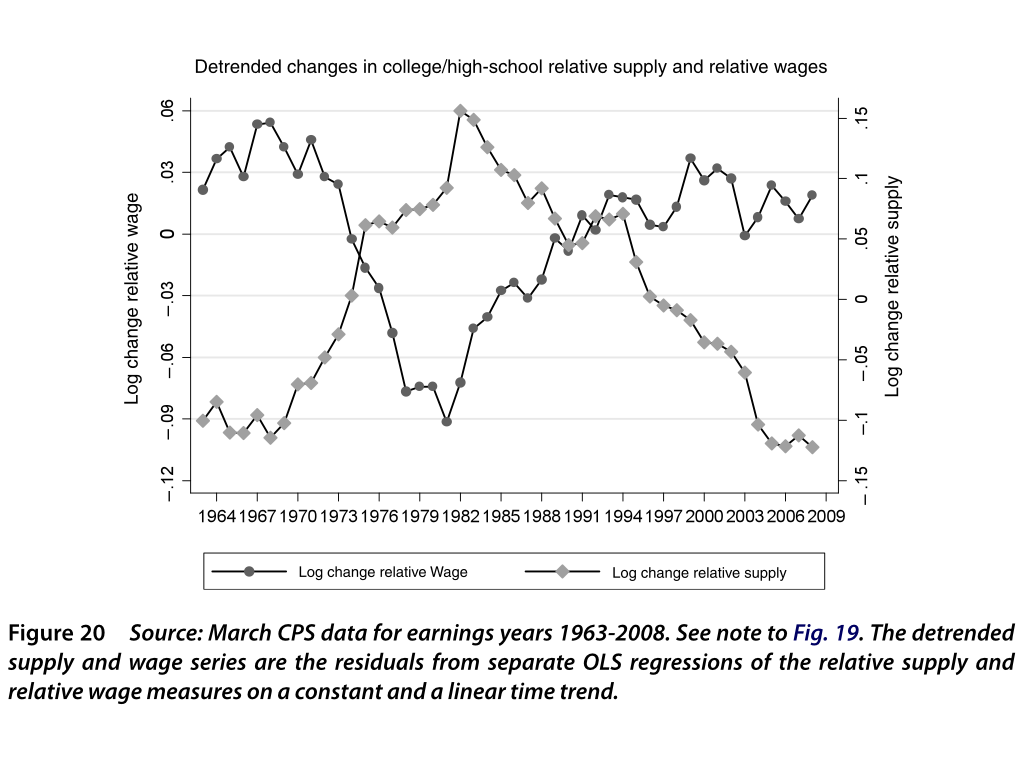
\includegraphics[height=8.5cm,width=\textwidth]{figure20.png}
\end{figure} 
\end{center}
\newpage

\newpage
\begin{center}
\begin{figure}
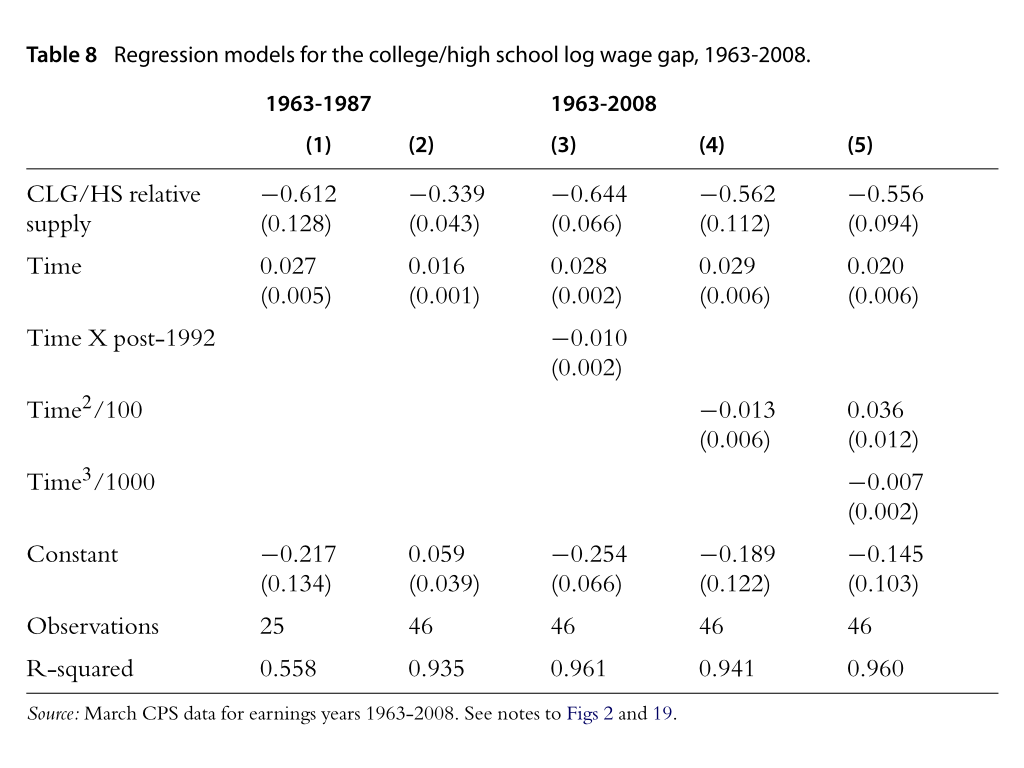
\includegraphics[height=8.5cm,width=\textwidth]{table8.png}
\end{figure} 
\end{center}
\newpage

\begin{frame}{Exploiting a richer set of facts}
\begin{itemize}
\item Additional identification and explanatory power can come from considering a richer set of facts. \medskip
\item Changes in the college premium were different by age groups: The college premium increased faster for younger workers in the early 1980s and for older workers in the late 1990s. \medskip
\item This could be because cohorts entering the labor market in the 1980s were relatively less educated and aged thereafter.
\end{itemize}
\end{frame}

\newpage
\begin{center}
\begin{figure}
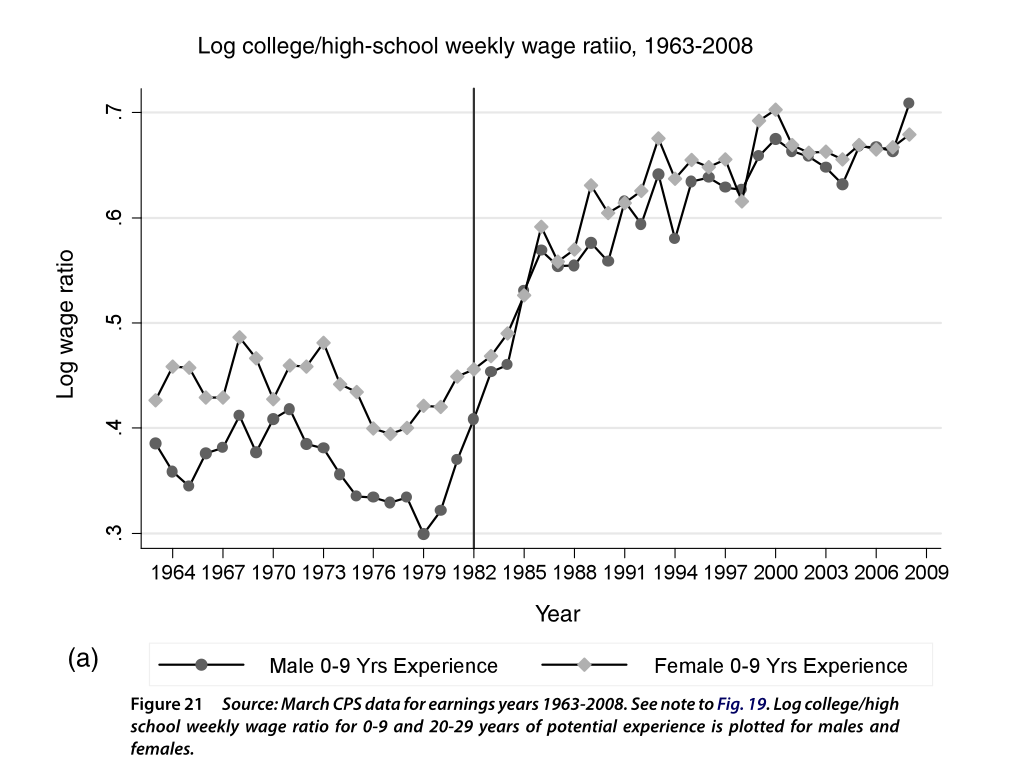
\includegraphics[height=8.5cm,width=\textwidth]{figure21a.png}
\end{figure} 
\end{center}
\newpage

\newpage
\begin{center}
\begin{figure}
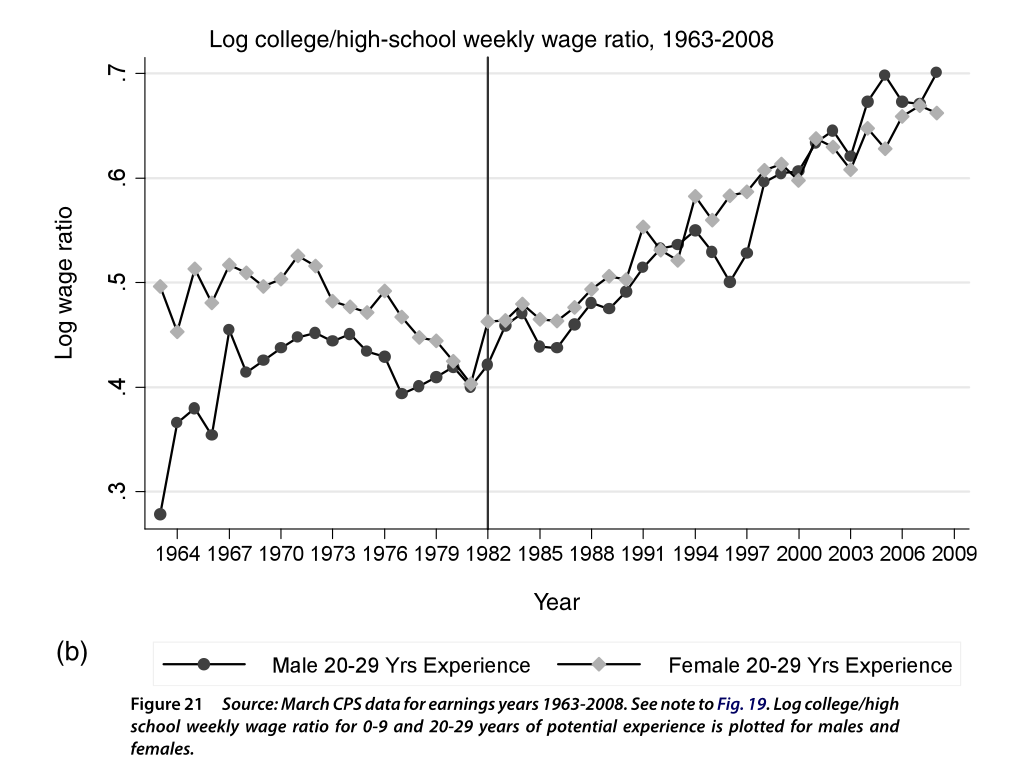
\includegraphics[height=8.5cm,width=\textwidth]{figure21b.png}
\end{figure} 
\end{center}
\newpage

\begin{frame}{An update of Card \& Lemieux [01]}
\begin{itemize}
\item Consider low ($L$) and high ($H$) skilled workers:
\[
Y=[L^{ \frac{\sigma_{e} -1}{\sigma_{e}}} + H^{ \frac{\sigma_{e} -1}{\sigma_{e}}}]^{\frac{\sigma_{e}}{\sigma_{e}-1}}
\]
with $L$ and $H$ aggregates across age groups $j$:
\[
L \equiv [\sum_{j}^{} L_{j}^{\frac{\sigma_{a} -1}{\sigma_{a}}}]^{\frac{\sigma_{a}}{\sigma_{a}-1}} \text{ and } 
H \equiv [\sum_{j}^{} H_{j}^{\frac{\sigma_{a} -1}{\sigma_{a}}}]^{\frac{\sigma_{a}}{\sigma_{a}-1}}
\]
\item Using the first-order conditions gives:
\[
\ln(\frac{w_{Hj}}{w_{Lj}})= - \frac{1}{\sigma_{a}}[\ln(\frac{H_{j}}{L_{j}})- \ln(\frac{H}{L})] - \frac{1}{\sigma_{e}} \ln(\frac{H}{L})
\]
\end{itemize}
\end{frame}

\begin{frame}{An update of Card \& Lemieux [01]}
\begin{itemize}
\item We had that (adding time subscripts $t$):
\[
\ln(\frac{w_{Hjt}}{w_{Ljt}})= - \frac{1}{\sigma_{a}}[ \ln(\frac{H_{jt}}{L_{jt}})- \ln(\frac{H_{t}}{L_{t}})] - \frac{1}{\sigma_{e}} \ln(\frac{H_{t}}{L_{t}})
\]
\item Adding a constant, a quadratic in time to capture SBTC, and a vector of age group main effects to capture persistent productivity differences between age groups:
\begin{align*}
\ln(\frac{w_{Hjt}}{w_{Ljt}})  = & \beta_{0} + \beta_{1} [ \ln(\frac{H_{jt}}{L_{jt}})- \ln(\frac{H_{t}}{L_{t}})] + \\
& \beta_{2} \ln(\frac{H_{t}}{L_{t}}) + \beta_{3}t + \beta_{4}t^{2} + \delta_{j} + \eta_{jt} 
\end{align*}
\end{itemize}
\end{frame}

\newpage
\begin{center}
\begin{figure}
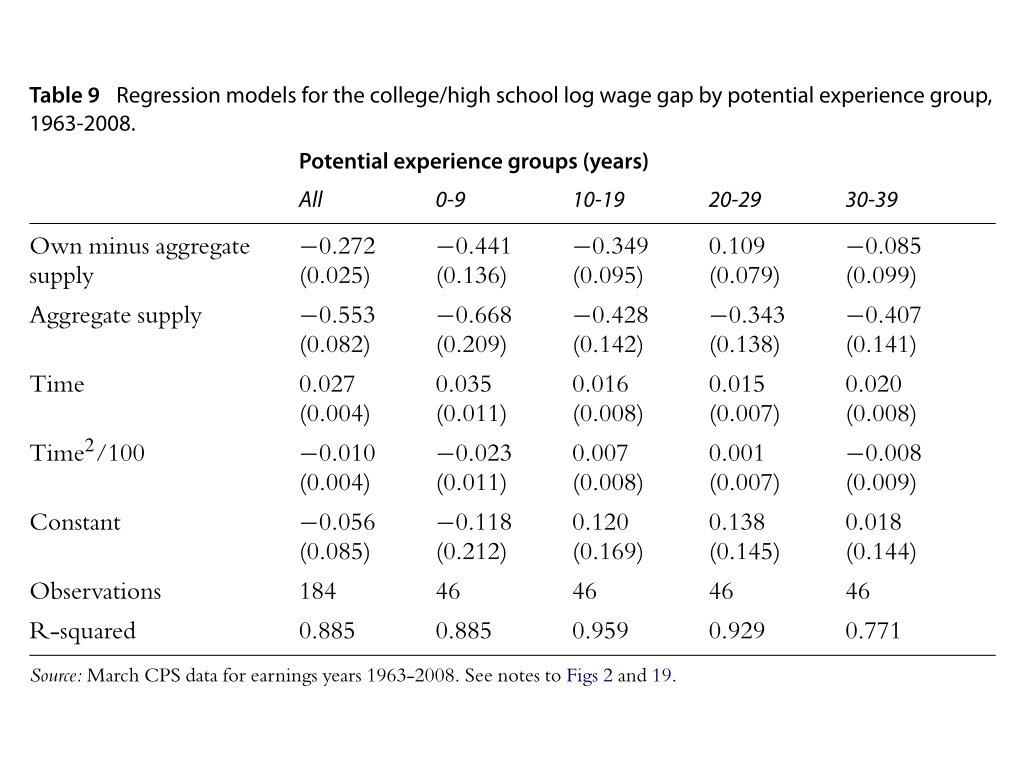
\includegraphics[height=8.5cm,width=\textwidth]{table9.png}
\end{figure} 
\end{center}
\newpage

\subsection{3.4 Overall inequality in the canonical model}

\begin{frame}{3. The canonical model}
\begin{itemize}
\item[\textcolor{gray}{3.1}] \textcolor{gray}{The simple theory of the canonical model} \medskip
\item[\textcolor{gray}{3.2}] \textcolor{gray}{Bringing Tinbergen's education race to the data} \medskip
\item[\textcolor{gray}{3.3}] \textcolor{gray}{Changes in earnings through the lens of the canonical model} \medskip
\item[\textcolor{red}{3.4}] \textcolor{red}{Overall inequality in the canonical model} \medskip
\item[\textcolor{gray}{3.5}] \textcolor{gray}{Endogenous change in technology} \medskip
\item[\textcolor{gray}{3.6}] \textcolor{gray}{Summary}
\end{itemize}
\end{frame}

\begin{frame}{Within-group wage inequality in the canonical model}
\begin{itemize}
\item The canonical model can also generate within-group wage inequality if there is heterogeneity in efficiency units:
\[
Y=\left[ [A_{L}L]^{\frac{\sigma -1}{\sigma }}+[A_{H}H]^{%
\frac{\sigma -1}{\sigma }}\right] ^{\frac{\sigma }{\sigma -1}} \tag{2}
\]
with $L=\int_{i\in \mathrm{L}}l_{i}di$ and $H=\int_{i\in \mathrm{H}}h_{i}di$.
\item Relative earnings of workers in the same group, say $\mathrm{L}$, are:
\[
\frac{W_{i}}{W_{i^{'}}} = \frac{w_{L}l_{i}}{w_{L}l_{i^{'}}} = \frac{l_{i}}{l_{i^{'}}} \text{ for } i,i^{'} \in \mathrm{L}
\]
\item Canonical model can generate within-group wage inequality, but this inequality is independent of the skill premium. 
\end{itemize}
\end{frame}

\begin{frame}{Overall inequality in the canonical model}
\begin{itemize}
\item Assume two observable skill groups of college ($C$) and non-college ($N$) workers. \medskip
\item Assume that a fraction $\phi_{c}$ of college workers and a fraction $ \phi_{n}$ of non-college workers are high-skilled ($H$) with the remaining fractions being low-skilled ($L$). \medskip
\item Denote the true skill wage premium by:
\[
\omega \equiv \frac{w_{H}}{w_{L}}
\]
\item Denote the observed college wage premium by:
\[
\omega^{c} \equiv \frac{w_{C}}{w_{N}}
\]
\end{itemize}
\end{frame}

\begin{frame}{Overall inequality in the canonical model}
\begin{itemize}
\item The observed college wage premium can be written as:
\[
\omega^{c} = \frac{w_{C}}{w_{N}} = \frac{\phi_{c}w_{H}+[1-\phi_c]w_{L}}{\phi_{n}w_{H}+[1-\phi_{n}]w_{L}} = \frac{\phi_{c} \omega + [1-\phi_c]}{\phi_{n} \omega +[1-\phi_{n}]}
\]
\item If $ \phi_{n} < \phi_{c}$, $ \omega^{c}$ is increasing in $ \omega $. \medskip
\item Denote the within-group skill premium by $ \omega^{\text{within}} = \omega $. \medskip
\item For constant $\phi_{c}$ and $\phi_{n}$,  $ \omega^{c}  $, $ \omega^{\text{within}} $ and $ \omega $ will move together. \medskip
\item The canonical model can predict changes in within-group and overall inequality (but not very intuitively).
\end{itemize}
\end{frame}

\subsection{3.5 Endogenous change in technology}

\begin{frame}{3. The canonical model}
\begin{itemize}
\item[\textcolor{gray}{3.1}] \textcolor{gray}{The simple theory of the canonical model} \medskip
\item[\textcolor{gray}{3.2}] \textcolor{gray}{Bringing Tinbergen's education race to the data} \medskip
\item[\textcolor{gray}{3.3}] \textcolor{gray}{Changes in earnings through the lens of the canonical model} \medskip
\item[\textcolor{gray}{3.4}] \textcolor{gray}{Overall inequality in the canonical model} \medskip
\item[\textcolor{red}{3.5}] \textcolor{red}{Endogenous change in technology} \medskip
\item[\textcolor{gray}{3.6}] \textcolor{gray}{Summary}
\end{itemize}
\end{frame}

\begin{frame}{Directed technological change}
\begin{itemize}
\item The canonical model assumes SBTC is a steady process that can be captured by a time trend. \medskip
\item However, the speed of technological change can be endogenous and directed by the relative supply of high-skill workers. \medskip
\item A more skilled workforce induces skill-biased technological change. \medskip
\item Steady SBTC could result from a steady increase in the supply of skills (thus uniting the two parts of Tinbergen's race). 
\end{itemize}
\end{frame}

\subsection{3.6 Summary}

\begin{frame}{3. The canonical model}
\begin{itemize}
\item[\textcolor{gray}{3.1}] \textcolor{gray}{The simple theory of the canonical model} \medskip
\item[\textcolor{gray}{3.2}] \textcolor{gray}{Bringing Tinbergen's education race to the data} \medskip
\item[\textcolor{gray}{3.3}] \textcolor{gray}{Changes in earnings through the lens of the canonical model} \medskip
\item[\textcolor{gray}{3.4}] \textcolor{gray}{Overall inequality in the canonical model} \medskip
\item[\textcolor{gray}{3.5}] \textcolor{gray}{Endogenous change in technology} \medskip
\item[\textcolor{red}{3.6}] \textcolor{red}{Summary}
\end{itemize}
\end{frame}

\begin{frame}{Summary}
\begin{itemize}
\item The canonical model provides a parsimonious framework for thinking about the changes skill premium and changes in overall wage inequality. \medskip
\item The canonical model has been very successful empirically. \medskip
\item It explains observed fluctuations in the skill premium by a secular increase in the relative demand for college workers due to SBTC combined with fluctuations in the growth of relative skill supplies. \medskip
\item However, the canonical model falls short of explaining several recent trends in advanced labor markets.
\end{itemize}
\end{frame}

\begin{frame}{Problem and puzzles for the canonical model}
\begin{itemize}
\item It does not provide an explanation why wages of unskilled workers have fallen (because it assumes q-complementarity). \medskip 
\item It does not explain the phenomenon of wage and job polarization (why demand for unskilled relative to middle skilled workers has increased). \medskip
\item It is at odds with the idea that technologies directly replace workers (automation instead of factor-augmenting technological change).
\item It is silent about the recent fall in the labor share. \medskip
\item It is not informative about the role of imperfections (because it is a simple supply-demand framework).
\end{itemize}
\end{frame}

\end{document}
